%\addtocontents{toc}{\setlength\cftchapternumwidth{1em}}
%\renewcommand\thechapter{}


\chapter{Trigger scale factors}
%\renewcommand{\thechapter}{A}
\label{app:TriggerSF}



The trigger scale factors measured as a function of lepton \pt, using the dataset collected by \Etmis\ triggers and \WZ\ simulation, after a 3 lepton and jets selection, in the Z mass window. All corrections to simulation are applied.



\begin{table}[htbp]
	\centering
	\caption{Trigger efficiencies on data events selected with \Etmis\ triggers and \WZ\ simulation for all lepton channels together. The unweighed number of events is quoted. When there are no events passing the cuts, it is indicated with N/A. The uncertainties are statistical uncertainties.}
	\begin{tabular}{c|c|c|c|c}
		\toprule
		ALL CHANNEL & \multicolumn{2}{c|}{data} & \multicolumn{2}{c}{WZ simulations} \\ 
		& Efficiency & unc. & Efficiency & unc. \\
		\midrule 
		3 lep,  at least one jet & 117/118 = 99.15 \% & 12.94\% & 18047/18055 = 99.96\%  & 1.05\% \\ 
		\hline 
		\STSR & 6/6 = 100.00\% & 57.74\% & 1541/1541 = 100.00\% & 3.60\% \\ 
		\hline 
		\TTSR & 26/27 = 96.30\% & 26.46\% & 1791/1792 = 99.94\% & 3.34\% \\ 
		\hline 
		\WZCR & 69/69 = 100.00 \% & 17.03\% & 14405/14412=99.95\% & 1.18\% \\ 
		\bottomrule 
	\end{tabular} 
\end{table}	
\begin{table}[htbp]
	\centering
	\caption{Trigger efficiencies on data events selected with \Etmis\ triggers and \WZ\ simulation for \mumumu\ lepton channel together. The unweighed number of events is quoted. When there are no events passing the cuts, it is indicated with N/A. The uncertainties are statistical uncertainties.}
	\begin{tabular}{c|c|c|c|c}
		\toprule 
		\mumumu\ CHANNEL & \multicolumn{2}{c|}{data} & \multicolumn{2}{c}{\WZ\ simulations} \\
		& Efficiency & unc. & Efficiency & unc. \\ 
		\midrule 
		3 lep,  at least one jet & 40/40 = 100.00 \% & 22.36 \% & 7814/7814 = 100.00\%  & 1.60\% \\ 
		\hline 
		\STSR & N/A & N/A & 687/687 = 100\% & 5.40\% \\ 
		\hline 
		\TTSR & 13/13 = 100.00\% & 39.22\% &763/763 = 100.00\% & 5.12\% \\ 
		\hline 
		\WZCR & 22/22 = 100.00 \% & 30.15\% & 6238/6238=100.00\% & 1.79\% \\ 
		\bottomrule
	\end{tabular} 
\end{table}	
\begin{table}[htbp]
	\centering
	\caption{Trigger efficiencies on data events selected with \Etmis\ triggers and \WZ\ simulation for \eee\ lepton channel together. The unweighed number of events is quoted. When there are no events passing the cuts, it is indicated with N/A. The uncertainties are statistical uncertainties.}

	\begin{tabular}{c|c|c|c|c}
		\toprule 
		\eee\ CHANNEL & \multicolumn{2}{c|}{data} & \multicolumn{2}{c}{WZ simulations} \\ 
		& Efficiency & unc. & Efficiency & unc. \\
		\midrule
		3 lep,  at least one jet & 20/21 = 95.24\%  & 29.76\% & 2211/2215 = 99.82 \% & 3.00\%  \\ 
		\hline 
		\STSR & 4/4 = 100.00\% & 70.71\% & 176/176 = 100.00\% & 10.66\% \\ 
		\hline 
		\TTSR & 2/3 = 66.67\% & 60.86\% & 242/242 = 100.00\% & 9.09\% \\ 
		\hline 
		\WZCR & 14/14 = 100.00 \% & 37.80\% & 1744/1748=99.77\% & 3.38\% \\ 
		\bottomrule
	\end{tabular} 
\end{table}
\begin{table}[htbp]
	\centering
	\caption{Trigger efficiencies on data events selected with \Etmis\ triggers and \WZ\ simulation for \eemu\ lepton channel together. The unweighed number of events is quoted. When there are no events passing the cuts, it is indicated with N/A. The uncertainties are statistical uncertainties.}

	\begin{tabular}{c|c|c|c|c}
		\toprule
		\eemu\ CHANNEL & \multicolumn{2}{c|}{data} & \multicolumn{2}{c}{WZ simulations} \\ 
		& Efficiency & unc. & Efficiency & unc. \\
		\midrule
		3 lep,  at least one jet & 32/32 = 100.00 \% & 25.00 \% & 3116/3118 = 99.94\%  & 2.53\% \\ 
		\hline 
		\STSR & 1/1 = 100.00\%& 141.42\% & 255/255 = 100\% & 8.86\% \\ 
		\hline 
		\TTSR & 9/9 = 100.00\% & 47.14\% &291/291 = 100.00\% & 8.29\% \\ 
		\hline 
		\WZCR & 14/14 = 100.00 \% & 37.80\% & 2529/2531=99.92\% & 2.81\% \\ 
		\bottomrule
	\end{tabular} 
\end{table}	
\begin{table}[htbp]
	\centering
	\caption{Trigger efficiencies on data events selected with \Etmis\ triggers and \WZ\ simulation for \emumu\ lepton channel together. The unweighed number of events is quoted. When there are no events passing the cuts, it is indicated with N/A. The uncertainties are statistical uncertainties.}

	\begin{tabular}{c|c|c|c|c}
		\toprule 
		\emumu\ CHANNEL & \multicolumn{2}{c|}{data} & \multicolumn{2}{c}{WZ simulations} \\ 
		& Efficiency & unc. & Efficiency & unc. \\
		\midrule
		3 lep,  at least one jet & 25/25 = 100.00\%  & 28.28\% & 4906/4908 = 99.96 \% & 2.02\%  \\ 
		\hline 
		\STSR & 1/1 = 100.00\% &141.42\% & 423/423 = 100.00\% & 6.88\% \\ 
		\hline 
		\TTSR & 2/2 = 100.00\% & 100.00\% & 495/496 = 99.80\% & 6.34\% \\ 
		\hline 
		\WZCR & 19/19 = 100.00 \% & 32.44\% & 3894/3895 =99.97\% & 2.27\% \\ 
		\bottomrule 
	\end{tabular} 
	\label{tab:trigSF}
\end{table}
\begin{comment}

\begin{figure}[tb]
	[In function of lepton \pt]{
		\includegraphics[width=0.48\textwidth]{Appendix/Figures/trigger/Triggereff/1e2mu/triggeff_1e2muhistPt.png}
		\label{image:triggeff_1e2muhistPt.png}
	}
	[In function of 2nd leading lepton in \pt]{
		\includegraphics[width=0.48\textwidth]{Appendix/Figures/trigger/Triggereff/1e2mu/triggeff_1e2muhistPt_2ndleadinglep.png}
		\label{image:triggeff_1e2muhistPt_2ndleadinglep.png}
	}
	\newline
	[In function of 3d leading lepton in \pt]{
		\includegraphics[width=0.48\textwidth]{Appendix/Figures/trigger/Triggereff/1e2mu/triggeff_1e2muhistPt_3dleadinglep.png}
		\label{image:triggeff_1e2muhistPt_3dleadinglep.png}
	}
	[In function of leading lepton in \pt]{
		\includegraphics[width=0.48\textwidth]{Appendix/Figures/trigger/Triggereff/1e2mu/triggeff_1e2muhistPt_leadinglep.png}
		\label{image:triggeff_1e2muhistPt_leadinglep.png}
	}
	\caption{The trigger efficiencies measured as a function of lepton \pt, using the dataset collected by \Etmis\ triggers and \WZ\ simulation, after a 3 lepton and jets selection, in the Z mass window. All corrections to simulation are applied. 1e2$\mu$ channel.}
	\label{image:FigurestriggerTriggereff1e2mu}
\end{figure}

\begin{figure}[tb]
	[In function of lepton \pt]{
		\includegraphics[width=0.48\textwidth]{Appendix/Figures/trigger/Triggereff/2e1mu/triggeff_2e1muhistPt.png}
		\label{image:triggeff_2e1muhistPt.png}
	}
	[In function of 2nd leading lepton in \pt]{
		\includegraphics[width=0.48\textwidth]{Appendix/Figures/trigger/Triggereff/2e1mu/triggeff_2e1muhistPt_2ndleadinglep.png}
		\label{image:triggeff_2e1muhistPt_2ndleadinglep.png}
	}
	\newline
	[In function of 3d leading lepton in \pt]{
		\includegraphics[width=0.48\textwidth]{Appendix/Figures/trigger/Triggereff/2e1mu/triggeff_2e1muhistPt_3dleadinglep.png}
		\label{image:triggeff_2e1muhistPt_3dleadinglep.png}
	}
	[In function of leading lepton in \pt]{
		\includegraphics[width=0.48\textwidth]{Appendix/Figures/trigger/Triggereff/2e1mu/triggeff_2e1muhistPt_leadinglep.png}
		\label{image:triggeff_2e1muhistPt_leadinglep.png}
	}
	\caption{The trigger efficiencies measured as a function of lepton \pt, using the dataset collected by \Etmis\ triggers and \WZ\ simulation, after a 3 lepton and jets selection, in the Z mass window. All corrections to simulation are applied. 2e1$\mu$ channel.}
	\label{image:FigurestriggerTriggereff2e1mu}
\end{figure}

\begin{figure}[tb]
	[In function of lepton \pt]{
		\includegraphics[width=0.48\textwidth]{Appendix/Figures/trigger/Triggereff/3e/triggeff_3ehistPt.png}
		\label{image:triggeff_3ehistPt.png}
	}
	[In function of 2nd leading lepton in \pt]{
		\includegraphics[width=0.48\textwidth]{Appendix/Figures/trigger/Triggereff/3e/triggeff_3ehistPt_2ndleadinglep.png}
		\label{image:triggeff_3ehistPt_2ndleadinglep.png}
	}
	\newline
	[In function of 3d leading lepton in \pt]{
		\includegraphics[width=0.48\textwidth]{Appendix/Figures/trigger/Triggereff/3e/triggeff_3ehistPt_3dleadinglep.png}
		\label{image:triggeff_3ehistPt_3dleadinglep.png}
	}
	[In function of leading lepton in \pt]{
		\includegraphics[width=0.48\textwidth]{Appendix/Figures/trigger/Triggereff/3e/triggeff_3ehistPt_leadinglep.png}
		\label{image:triggeff_3ehistPt_leadinglep.png}
	}
	\caption{The trigger efficiencies measured as a function of lepton \pt, using the dataset collected by \Etmis\ triggers and \WZ\ simulation, after a 3 lepton and jets selection, in the Z mass window. All corrections to simulation are applied. 3e channel.}
	\label{image:FigurestriggerTriggereff3e}
\end{figure}

\begin{figure}[tb]
	[In function of lepton \pt]{
		\includegraphics[width=0.48\textwidth]{Appendix/Figures/trigger/Triggereff/3mu/triggeff_3muhistPt.png}
		\label{image:triggeff_3muhistPt.png}
	}
	[In function of 2nd leading lepton in \pt]{
		\includegraphics[width=0.48\textwidth]{Appendix/Figures/trigger/Triggereff/3mu/triggeff_3muhistPt_2ndleadinglep.png}
		\label{image:triggeff_3muhistPt_2ndleadinglep.png}
	}
	\newline
	[In function of 3d leading lepton in \pt]{
		\includegraphics[width=0.48\textwidth]{Appendix/Figures/trigger/Triggereff/3mu/triggeff_3muhistPt_3dleadinglep.png}
		\label{image:triggeff_3muhistPt_3dleadinglep.png}
	}
	[In function of leading lepton in \pt]{
		\includegraphics[width=0.48\textwidth]{Appendix/Figures/trigger/Triggereff/3mu/triggeff_3muhistPt_leadinglep.png}
		\label{image:triggeff_3muhistPt_leadinglep.png}
	}
	\caption{The trigger efficiencies measured as a function of lepton \pt, using the dataset collected by \Etmis\ triggers and \WZ\ simulation, after a 3 lepton and jets selection, in the Z mass window. All corrections to simulation are applied. 3$\mu$ channel.}
	\label{image:FigurestriggerTriggereff3mu}
\end{figure}

\begin{figure}[tb]
	[In function of lepton \pt]{
		\includegraphics[width=0.48\textwidth]{Appendix/Figures/trigger/Triggereff/all/triggeff_allhistPt.png}
		\label{image:triggeff_allhistPt.png}
	}
	[In function of 2nd leading lepton in \pt]{
		\includegraphics[width=0.48\textwidth]{Appendix/Figures/trigger/Triggereff/all/triggeff_allhistPt_2ndleadinglep.png}
		\label{image:triggeff_allhistPt_2ndleadinglep.png}
	}
	\newline
	[In function of 3d leading lepton in \pt]{
		\includegraphics[width=0.48\textwidth]{Appendix/Figures/trigger/Triggereff/all/triggeff_allhistPt_3dleadinglep.png}
		\label{image:triggeff_allhistPt_3dleadinglep.png}
	}
	[In function of leading lepton in \pt]{
		\includegraphics[width=0.48\textwidth]{Appendix/Figures/trigger/Triggereff/all/triggeff_allhistPt_leadinglep.png}
		\label{image:triggeff_allhistPt_leadinglep.png}
	}
	\caption{The trigger efficiencies measured as a function of lepton \pt, using the dataset collected by \Etmis\ triggers and \WZ\ simulation, after a 3 lepton and jets selection, in the Z mass window. All corrections to simulation are applied. All channel.}
	\label{image:FigurestriggerTriggereffall}
\end{figure}

\begin{figure}[tb]
	[In function of lepton \pt]{
		\includegraphics[width=0.48\textwidth]{Appendix/Figures/trigger/ScaleFactors/1e2mu/SF_trigger_1e2muhistPt.png}
		\label{image:1e2muhistPt.png}
	}
	[In function of 2nd leading lepton in \pt]{
		\includegraphics[width=0.48\textwidth]{Appendix/Figures/trigger/ScaleFactors/1e2mu/SF_trigger_1e2muhistPt_2ndleadinglep.png}
		\label{image:1e2muhistPt_2ndleadinglep.png}
	}
	\newline
	[In function of 3d leading lepton in \pt]{
		\includegraphics[width=0.48\textwidth]{Appendix/Figures/trigger/ScaleFactors/1e2mu/SF_trigger_1e2muhistPt_3dleadinglep.png}
		\label{image:1e2muhistPt_3dleadinglep.png}
	}
	[In function of leading lepton in \pt]{
		\includegraphics[width=0.48\textwidth]{Appendix/Figures/trigger/ScaleFactors/1e2mu/SF_trigger_1e2muhistPt_leadinglep.png}
		\label{image:1e2muhistPt_leadinglep.png}
	}
	\caption{The trigger scale factors measured as a function of lepton \pt, using the dataset collected by \Etmis\ triggers and \WZ\ simulation, after a 3 lepton and jets selection, in the Z mass window. All corrections to simulation are applied. 1e2$\mu$ channel.}
	\label{image:FigurestriggerScaleFactors1e2mu}
\end{figure}

\begin{figure}[tb]
	[In function of lepton \pt]{
		\includegraphics[width=0.48\textwidth]{Appendix/Figures/trigger/ScaleFactors/2e1mu/SF_trigger_2e1muhistPt.png}
		\label{image:2e1muhistPt.png}
	}
	[In function of 2nd leading lepton in \pt]{
		\includegraphics[width=0.48\textwidth]{Appendix/Figures/trigger/ScaleFactors/2e1mu/SF_trigger_2e1muhistPt_2ndleadinglep.png}
		\label{image:2e1muhistPt_2ndleadinglep.png}
	}
	\newline
	[In function of 3d leading lepton in \pt]{
		\includegraphics[width=0.48\textwidth]{Appendix/Figures/trigger/ScaleFactors/2e1mu/SF_trigger_2e1muhistPt_3dleadinglep.png}
		\label{image:2e1muhistPt_3dleadinglep.png}
	}
	[In function of leading lepton in \pt]{
		\includegraphics[width=0.48\textwidth]{Appendix/Figures/trigger/ScaleFactors/2e1mu/SF_trigger_2e1muhistPt_leadinglep.png}
		\label{image:2e1muhistPt_leadinglep.png}
	}
	\caption{The trigger scale factors measured as a function of lepton \pt, using the dataset collected by \Etmis\ triggers and \WZ\ simulation, after a 3 lepton and jets selection, in the Z mass window. All corrections to simulation are applied. 2e1$\mu$ channel.}
	\label{image:FigurestriggerScaleFactors2e1mu}
\end{figure}

\begin{figure}[tb]
	[In function of lepton \pt]{
		\includegraphics[width=0.48\textwidth]{Appendix/Figures/trigger/ScaleFactors/3e/SF_trigger_3ehistPt.png}
		\label{image:3ehistPt.png}
	}
	[In function of 2nd leading lepton in \pt]{
		\includegraphics[width=0.48\textwidth]{Appendix/Figures/trigger/ScaleFactors/3e/SF_trigger_3ehistPt_2ndleadinglep.png}
		\label{image:3ehistPt_2ndleadinglep.png}
	}
	\newline
	[In function of 3d leading lepton in \pt]{
		\includegraphics[width=0.48\textwidth]{Appendix/Figures/trigger/ScaleFactors/3e/SF_trigger_3ehistPt_3dleadinglep.png}
		\label{image:3ehistPt_3dleadinglep.png}
	}
	[In function of leading lepton in \pt]{
		\includegraphics[width=0.48\textwidth]{Appendix/Figures/trigger/ScaleFactors/3e/SF_trigger_3ehistPt_leadinglep.png}
		\label{image:3ehistPt_leadinglep.png}
	}
	\caption{The trigger scale factors measured as a function of lepton \pt, using the dataset collected by \Etmis\ triggers and \WZ\ simulation, after a 3 lepton and jets selection, in the Z mass window. All corrections to simulation are applied. 3e channel.}
	\label{image:FigurestriggerScaleFactors3e}
\end{figure}

\begin{figure}[tb]
	[In function of lepton \pt]{
		\includegraphics[width=0.48\textwidth]{Appendix/Figures/trigger/ScaleFactors/3mu/SF_trigger_3muhistPt.png}
		\label{image:3muhistPt.png}
	}
	[In function of 2nd leading lepton in \pt]{
		\includegraphics[width=0.48\textwidth]{Appendix/Figures/trigger/ScaleFactors/3mu/SF_trigger_3muhistPt_2ndleadinglep.png}
		\label{image:3muhistPt_2ndleadinglep.png}
	}
	\newline
	[In function of 3d leading lepton in \pt]{
		\includegraphics[width=0.48\textwidth]{Appendix/Figures/trigger/ScaleFactors/3mu/SF_trigger_3muhistPt_3dleadinglep.png}
		\label{image:3muhistPt_3dleadinglep.png}
	}
	[In function of leading lepton in \pt]{
		\includegraphics[width=0.48\textwidth]{Appendix/Figures/trigger/ScaleFactors/3mu/SF_trigger_3muhistPt_leadinglep.png}
		\label{image:3muhistPt_leadinglep.png}
	}
	\caption{The trigger scale factors measured as a function of lepton \pt, using the dataset collected by \Etmis\ triggers and \WZ\ simulation, after a 3 lepton and jets selection, in the Z mass window. All corrections to simulation are applied. 3$\mu$ channel.}
	\label{image:FigurestriggerScaleFactors3mu}
\end{figure}

\begin{figure}[tb]
	[In function of lepton \pt]{
		\includegraphics[width=0.48\textwidth]{Appendix/Figures/trigger/ScaleFactors/all/SF_trigger_allhistPt.png}
		\label{image:allhistPt.png}
	}
	[In function of 2nd leading lepton in \pt]{
		\includegraphics[width=0.48\textwidth]{Appendix/Figures/trigger/ScaleFactors/all/SF_trigger_allhistPt_2ndleadinglep.png}
		\label{image:allhistPt_2ndleadinglep.png}
	}
	\newline
	[In function of 3d leading lepton in \pt]{
		\includegraphics[width=0.48\textwidth]{Appendix/Figures/trigger/ScaleFactors/all/SF_trigger_allhistPt_3dleadinglep.png}
		\label{image:allhistPt_3dleadinglep.png}
	}
	[In function of leading lepton in \pt]{
		\includegraphics[width=0.48\textwidth]{Appendix/Figures/trigger/ScaleFactors/all/SF_trigger_allhistPt_leadinglep.png}
		\label{image:allhistPt_leadinglep.png}
	}
	\caption{The trigger scale factors measured as a function of lepton \pt, using the dataset collected by \Etmis\ triggers and \WZ\ simulation, after a 3 lepton and jets selection, in the Z mass window. All corrections to simulation are applied. All channel.}
	\label{image:FigurestriggerScaleFactorsall}
\end{figure}
\end{comment}

%\chapter{Dilepton controlplots}
%\label{app:controldilep}


\chapter{Transfer factors}
\label{app:tablestr}

	\begin{table}[htbp]
	\begin{center}
				\caption{Transfer factors for all lepton channels for going fro m \WZCR\ to the signal regions.  The transfer factors  $Tr_{\TTCR \rightarrow \TTSR}$  and $Tr_{\STCR \rightarrow \STSR}$ are 0.33.}
		
		\begin{tabular} {l cc}
			\toprule
			&$Tr_{\WZCR \rightarrow \STSR}$ & $Tr_{\WZCR \rightarrow \TTSR}$  \\ 
			\midrule
			\textbf{\kZut} &  0.22 $\pm $ 0.00 & 0.46 $\pm $ 0.00 \\ 
			\textbf{\kZct}  & 0.39 $\pm $ 0.01 & 0.76 $\pm $ 0.01 \\ 
			\textbf{\DY } & 0.08 $\pm $ 0.09 & 0.10 $\pm $ 0.10 \\ 
			\textbf{\ttbar}  & 0.54 $\pm $ 0.31 & 0.70 $\pm $ 0.31  \\  
			\textbf{\WZ} &  0.10 $\pm $ 0.00 & 0.15 $\pm $ 0.00 \\ 
			\textbf{\tZq} &0.36 $\pm $ 0.02 & 0.67 $\pm $ 0.03 \\ 
			\textbf{\ttZ} & 0.14 $\pm $ 0.02 & 0.61 $\pm $ 0.05 \\ 
			\textbf{\ZZ} & 0.10 $\pm $ 0.00 & 0.13 $\pm $ 0.00 \\ 
			\textbf{other} & 0.16 $\pm $ 0.03 & 0.30 $\pm $ 0.03 \\ 
			\bottomrule 
		\end{tabular}
	\end{center}
\end{table}


	
	\begin{table}[htbp]
		\begin{center}
						\caption{Event yields for the \ttbar\ background in all lepton channels. The yields below the dashed lines shoud be compared with the two first rows. }
			
			\begin{tabular} {l c}
				\toprule
				Region & \ttbar\ event yield  \\ 
				\midrule 
				\STSR & 13.1 $\pm $ 2.5 \\
				\TTSR & 9.7 $\pm $ 2.1 \\
				\TTCR & 22.3 $\pm $ 3.1 \\
				\STCR & 33.7 $\pm $ 3.8 \B\\
				\hdashline
				\TTSR\ (TTCR) & 7.44 $\pm $ 1.02 \T \\
				\STSR\ (STCR)& 11.24 $\pm $ 1.28 \\  				 
				\bottomrule
			\end{tabular}
		\end{center}
	\end{table}
\clearpage
\begin{landscape}
	\vspace*{\fill}
	\begin{table}[htb!]
	\begin{center}
				\caption{Event yields for all lepton channels. The last two columns represent the predicted event yield after applying the transfer factors. The regions between brackets correspond to the region from which the prediction is made.}
		
		\begin{tabular} {l ccccc|cc}
			\toprule
			& \STSR & \TTSR & \WZCR & \TTCR & \STCR & \STSR\ (\WZCR) & \TTSR\ (\WZCR)  \\ 
			\midrule 
			\textbf{\kZut} & 3.9 $\pm $0.0 & 11.2 $\pm $0.0 & 7.3 $\pm $0.0 & 0.6 $\pm $0.0 & 0.3 $\pm $0.0 & 1.57 $\pm $0.02 & 3.33 $\pm $0.04 \\ 
			\textbf{\kZct} & 14.1 $\pm $0.1 & 30.9 $\pm $0.1 & 15.5 $\pm $0.1 & 1.7 $\pm $0.0 & 1.2 $\pm $0.0 & 6.12 $\pm $0.08 & 11.77 $\pm $0.13 \\ 
			\textbf{\DY } & -4.6 $\pm $21.7 & 22.3 $\pm $14.3 & 136.9 $\pm $48.5 & -14.0 $\pm $22.2 & -15.9 $\pm $11.3 & 10.61 $\pm $11.31 & 13.69 $\pm $14.68 \\ 
			\textbf{\ttbar} & 13.1 $\pm $2.5 & 9.7 $\pm $2.1 & 8.5 $\pm $1.9 & 22.3 $\pm $3.1 & 33.7 $\pm $3.8 & 4.61 $\pm $2.37 & 5.89 $\pm $2.96  \\  
			\textbf{\WZ} & 60.9 $\pm $1.6 & 83.0 $\pm $1.7 & 552.7 $\pm $4.6 & 11.9 $\pm $0.6 & 8.5 $\pm $0.6 & 55.86 $\pm $1.57 & 83.80 $\pm $2.30 \\ 
			\textbf{\tZq} & 8.0 $\pm $0.2 & 16.9 $\pm $0.2 & 7.3 $\pm $0.2 & 2.2 $\pm $0.1 & 1.0 $\pm $0.1 & 2.66 $\pm $0.14 & 4.86 $\pm $0.25 \\ 
			\textbf{\ttZ} & 3.5 $\pm $0.3 & 42.5 $\pm $0.9 & 9.6 $\pm $0.5 & 6.8 $\pm $0.4 & 0.5 $\pm $0.1 & 1.37 $\pm $0.18 & 5.90 $\pm $0.59 \\ 
			\textbf{\ZZ} & 4.6 $\pm $0.1 & 4.8 $\pm $0.1 & 46.2 $\pm $0.3 & 0.8 $\pm $0.0 & 0.6 $\pm $0.0 & 4.48 $\pm $0.16 & 6.06 $\pm $0.21 \\ 
			\textbf{other} & 1.2 $\pm $0.3 & 5.6 $\pm $0.3 & 6.8 $\pm $0.5 & 7.5 $\pm $0.7 & 2.4 $\pm $0.5 & 1.09 $\pm $0.18 & 2.05 $\pm $0.24 \\ 
			\bottomrule
		\end{tabular}
	\end{center}
\end{table}
\vspace*{\fill}
\end{landscape}
\clearpage
\chapter{Details about the BDTs}
\label{app:BDTtechnics}
The boosted decision are trained without the \NPL\ background. In the following figures, the correlation matrices for the background and signal samples are shown. Furthermore, the resulting discriminating variables for background (red) and signal (blue) are shown. The ROC curves, illustrating the discriminating power of each discriminator is also shown for the training samples. At the bottom of each figure, the input variables used to train that discriminator are shown, where the background is shown in red and the signal in blue.
\begin{figure}[htbp]
	\includegraphics[width=0.48\textwidth]{6_Search/Figures/MVAtechnics/toppairzct/eee/CorrelationMatrixB.png}
	\includegraphics[width=0.48\textwidth]{6_Search/Figures/MVAtechnics/toppairzct/eee/CorrelationMatrixS.png}
	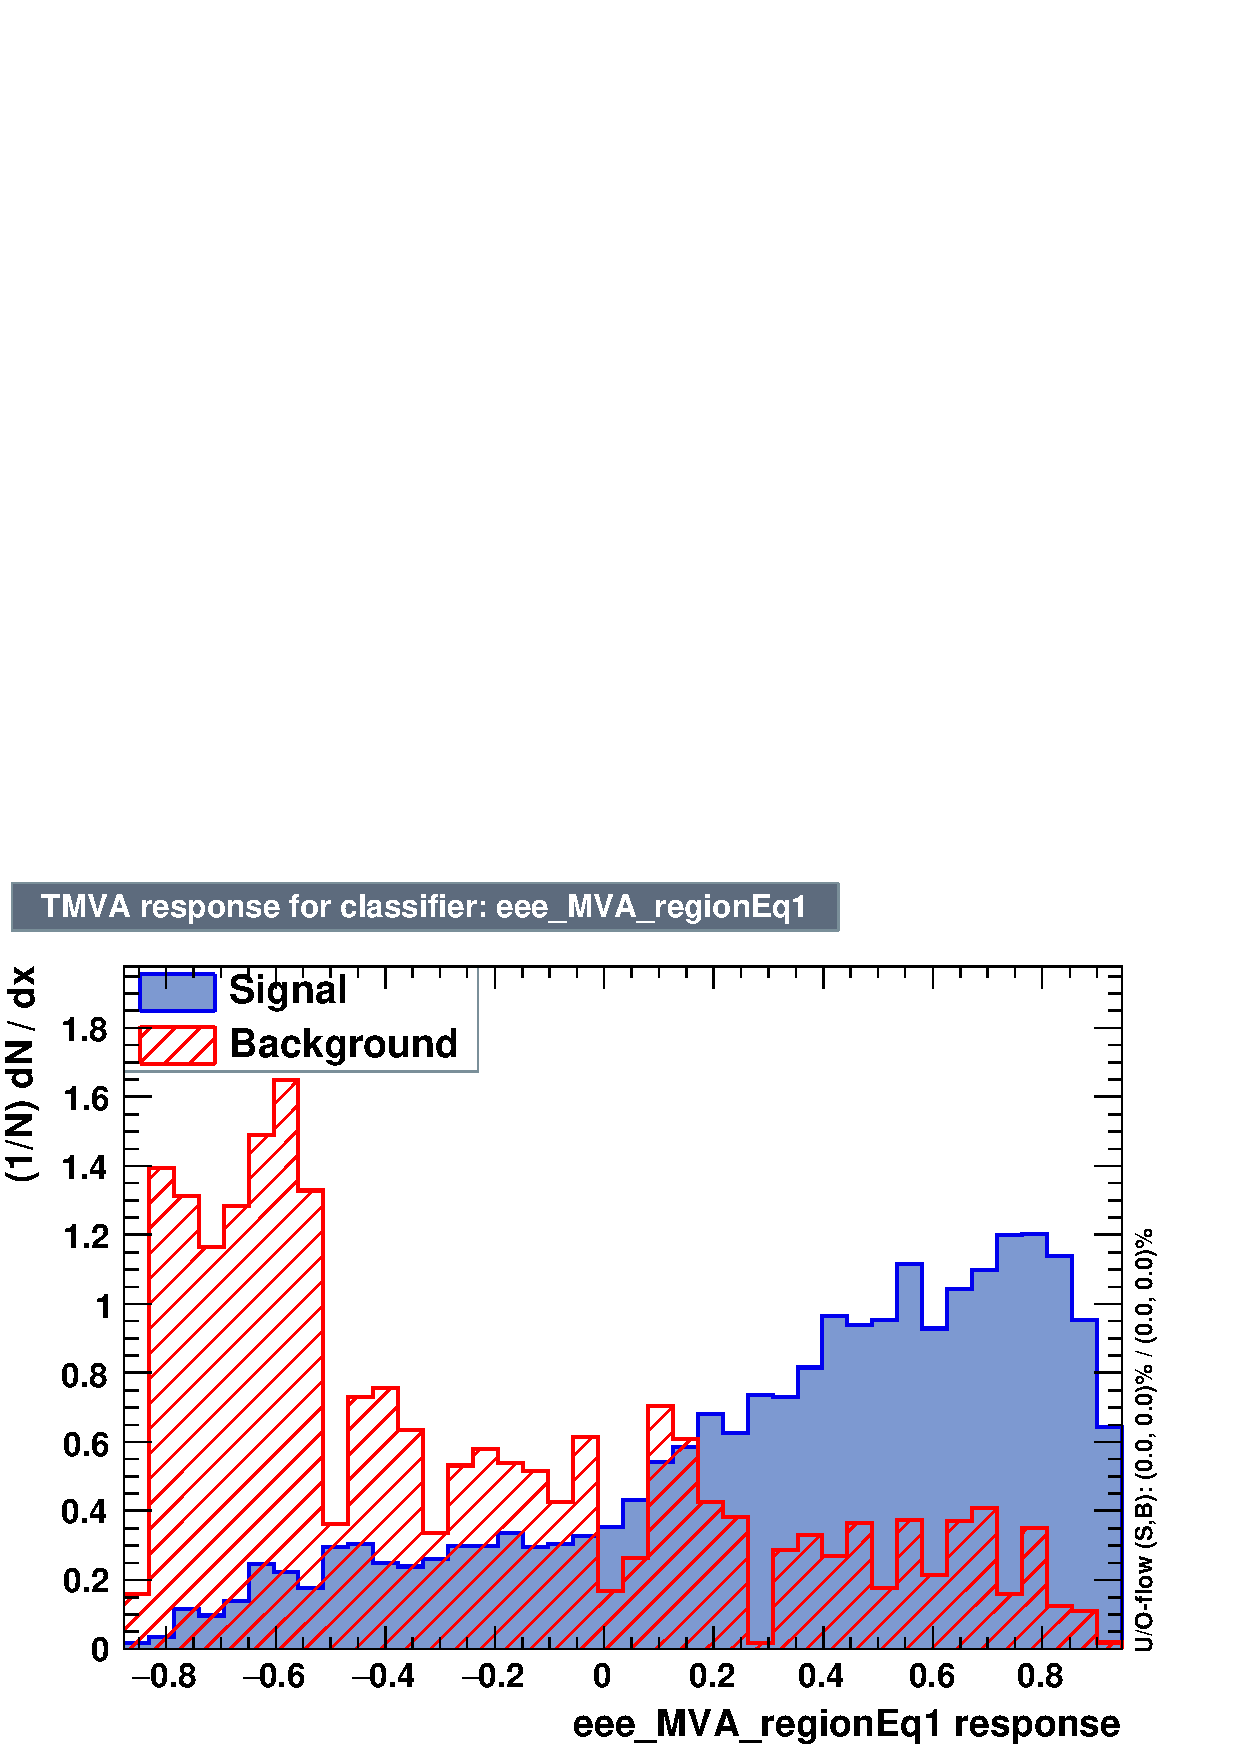
\includegraphics[width=0.48\textwidth]{6_Search/Figures/MVAtechnics/toppairzct/eee/mva_eee_MVA_regionEq1.png}
	\includegraphics[width=0.48\textwidth]{6_Search/Figures/MVAtechnics/toppairzct/eee/rejBvsS.png}
	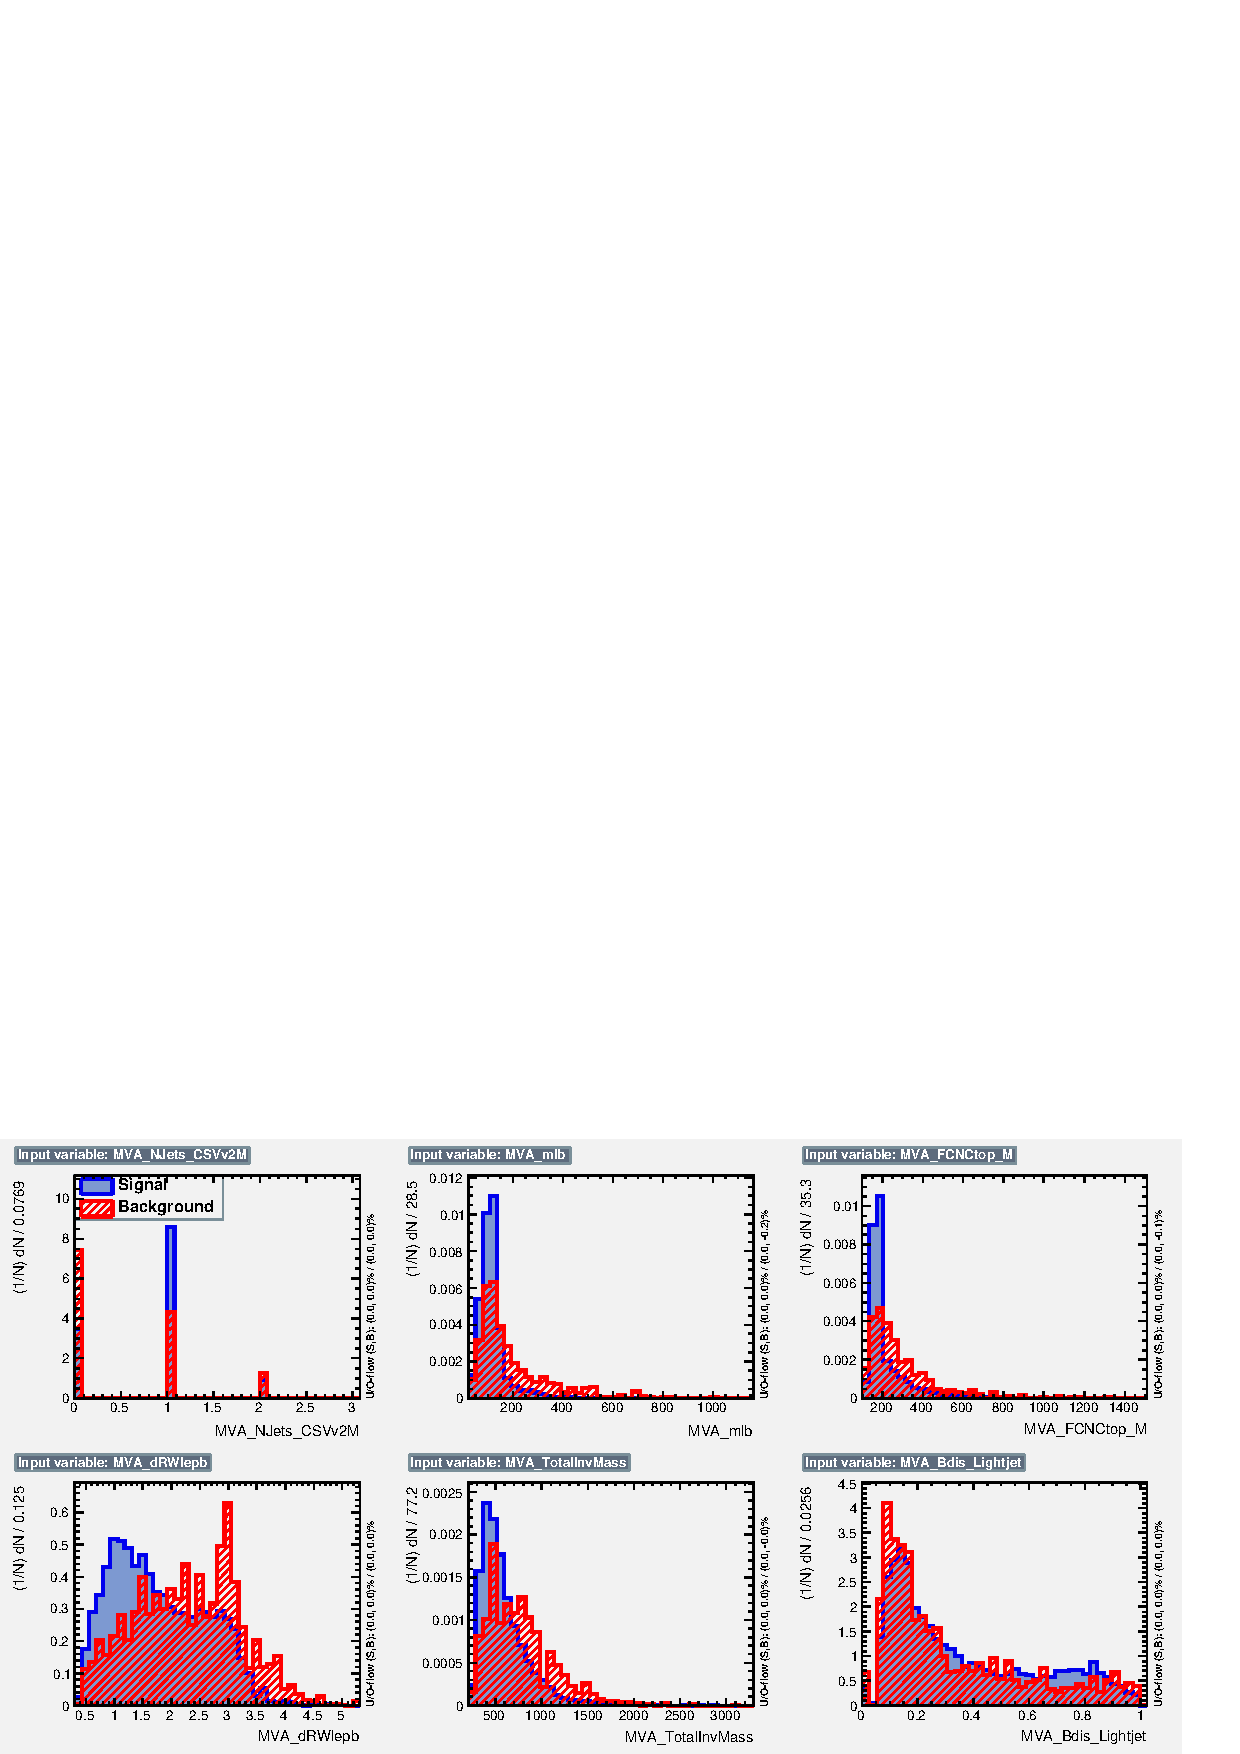
\includegraphics[width=0.48\textwidth]{6_Search/Figures/MVAtechnics/toppairzct/eee/variables_id_c1.png}
	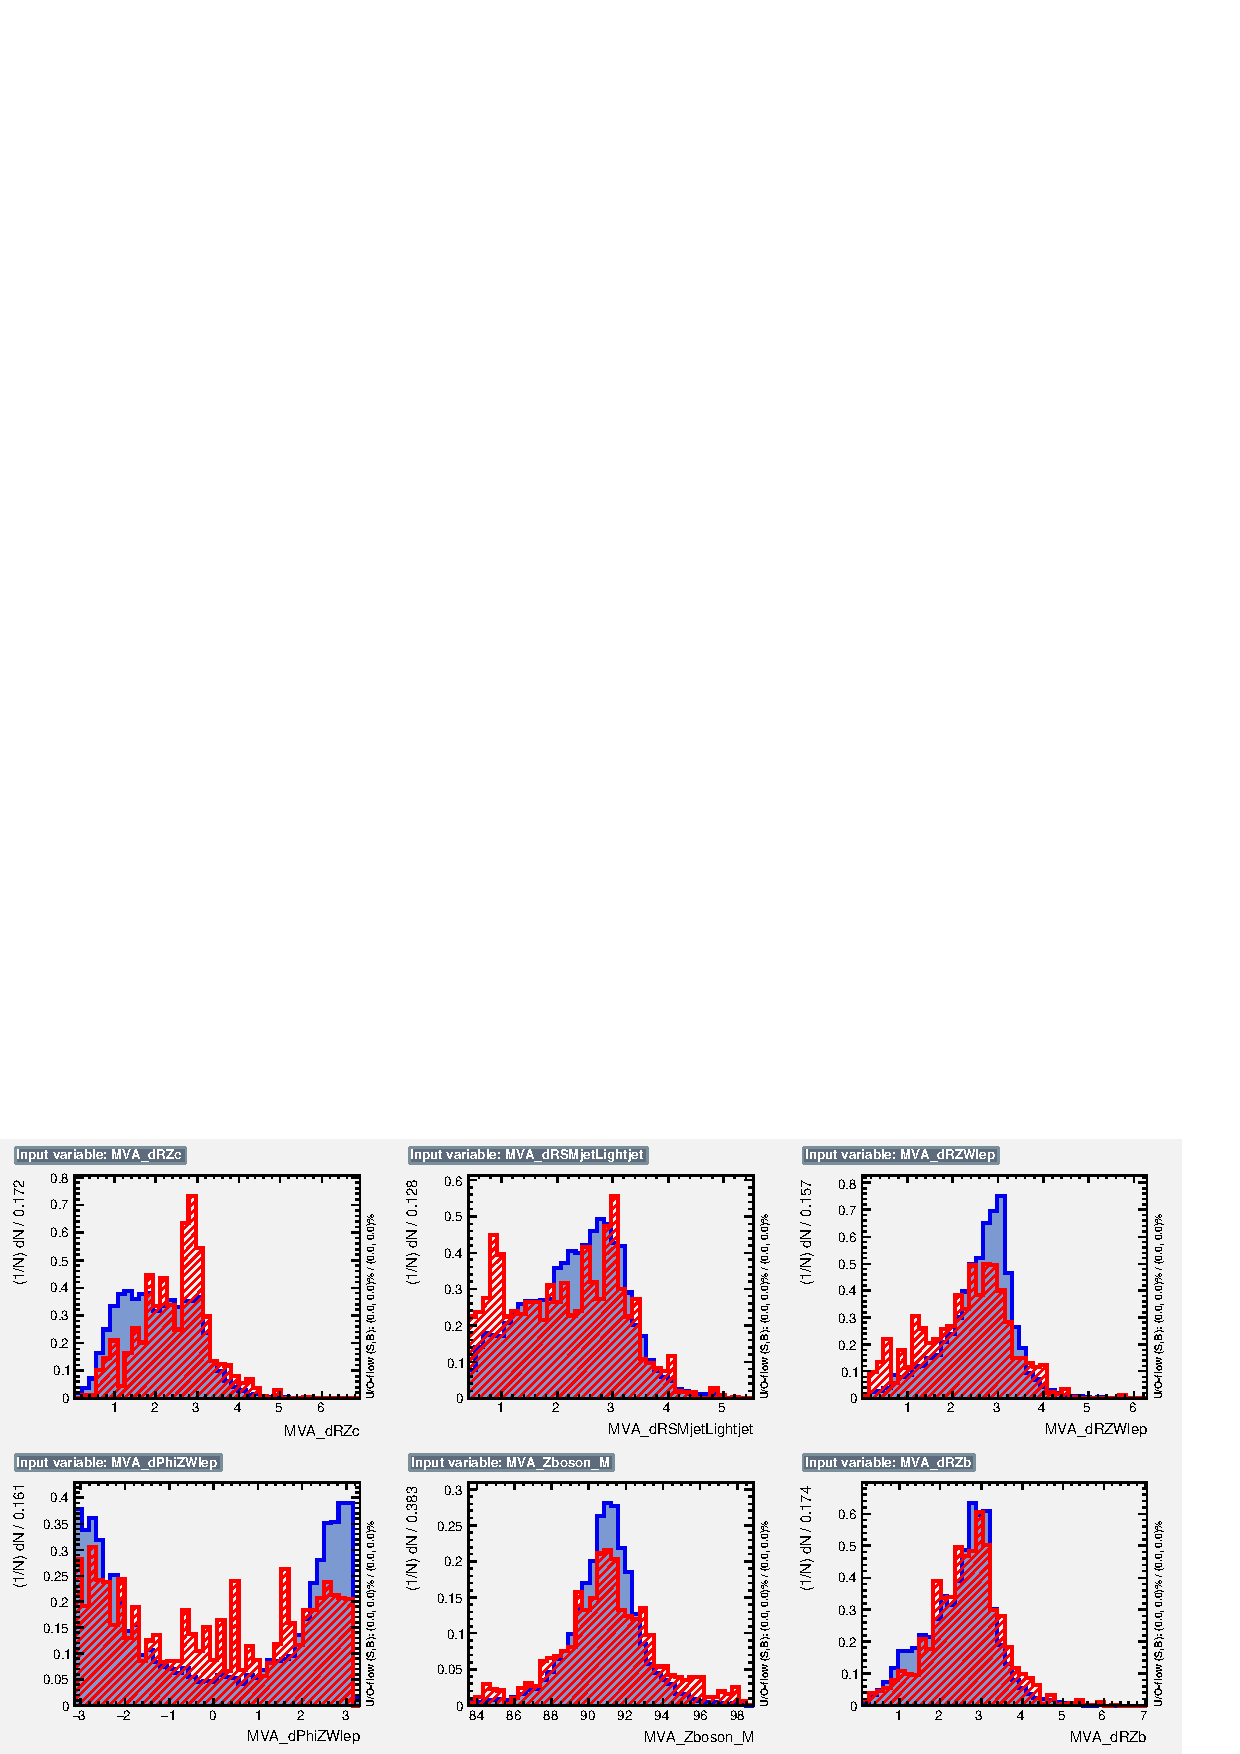
\includegraphics[width=0.48\textwidth]{6_Search/Figures/MVAtechnics/toppairzct/eee/variables_id_c2.png}
	\caption{\eee\ channel. \TTSR: \Zct\ vertex }
	\label{image:Figures3etoppairzct}
\end{figure}

\begin{figure}[htbp]
	\includegraphics[width=0.48\textwidth]{6_Search/Figures/MVAtechnics/toppairzct/eeu/CorrelationMatrixB.png}
	\includegraphics[width=0.48\textwidth]{6_Search/Figures/MVAtechnics/toppairzct/eeu/CorrelationMatrixS.png}
	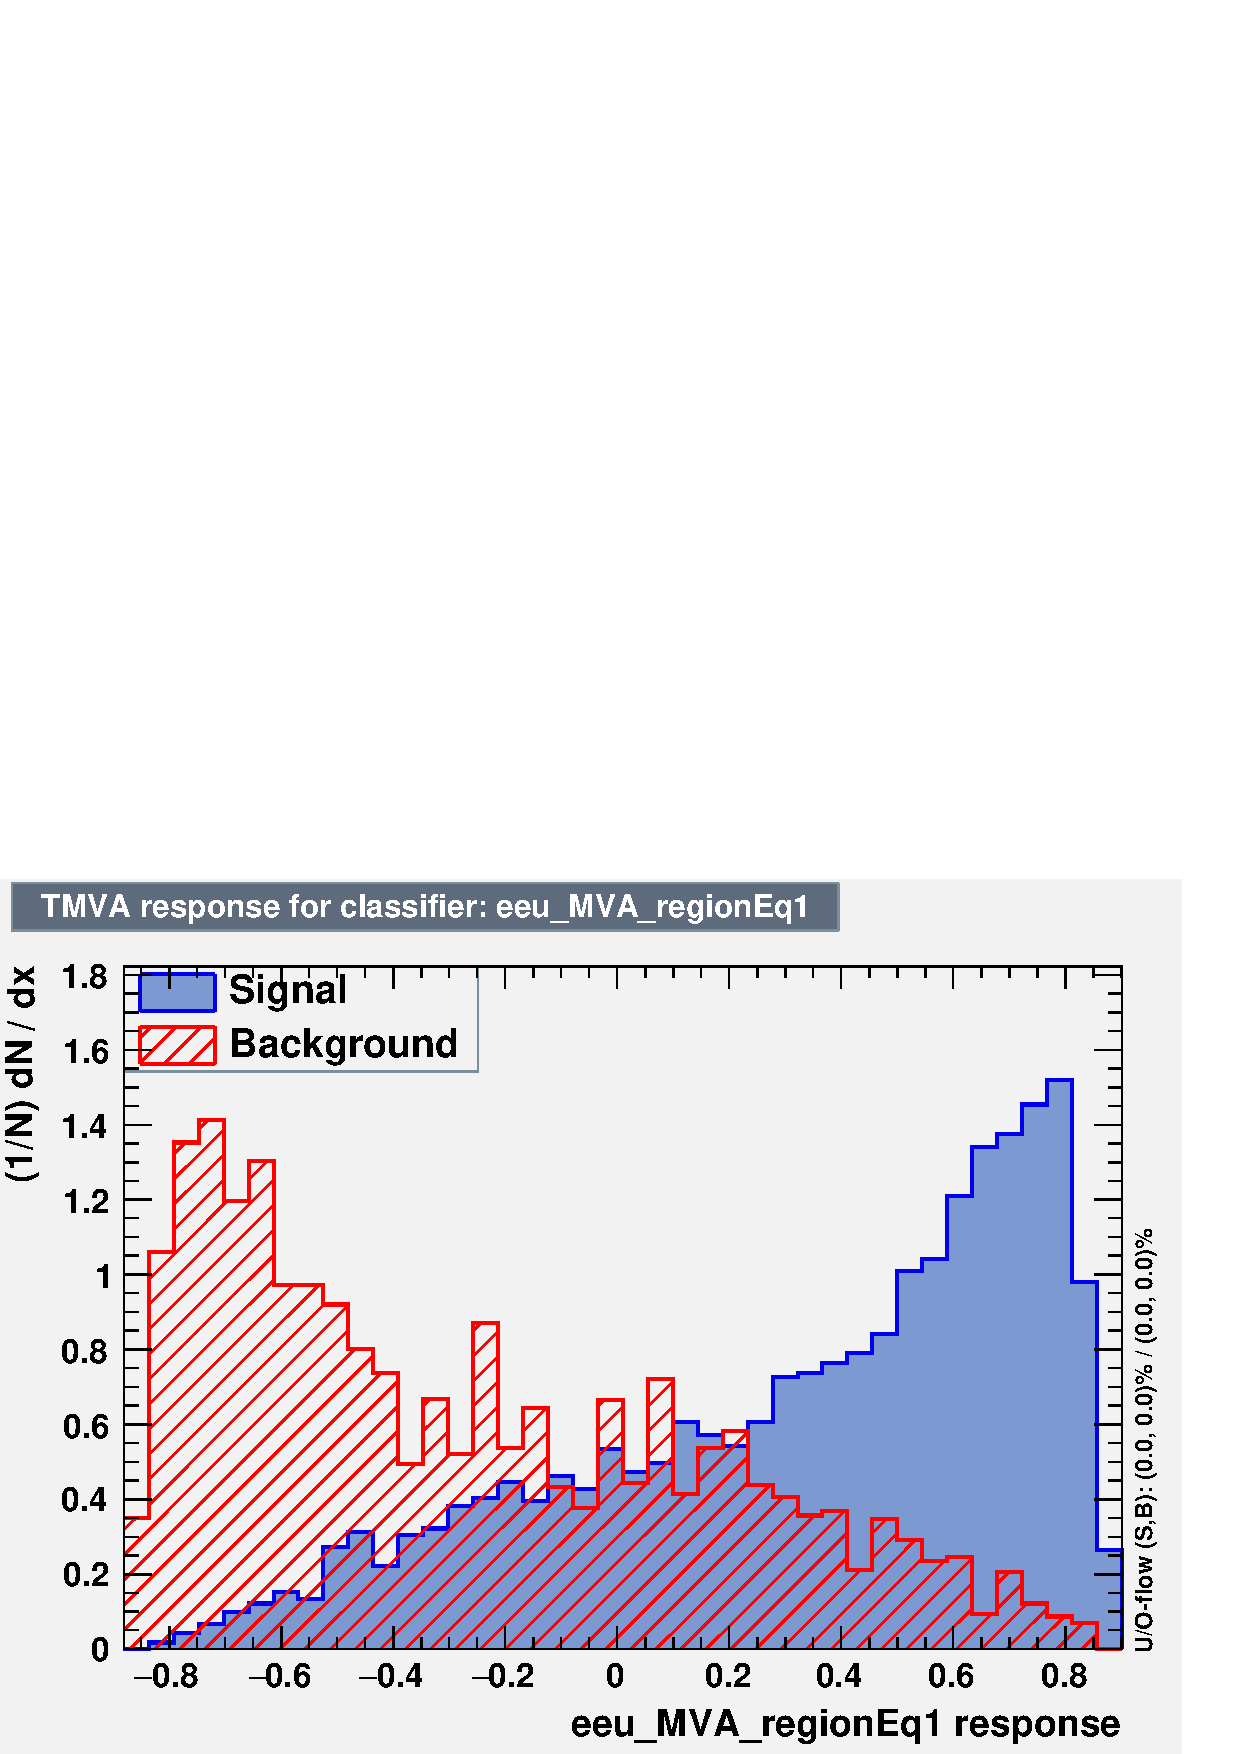
\includegraphics[width=0.48\textwidth]{6_Search/Figures/MVAtechnics/toppairzct/eeu/mva_eeu_MVA_regionEq1.png}
	\includegraphics[width=0.48\textwidth]{6_Search/Figures/MVAtechnics/toppairzct/eeu/rejBvsS.png}
	\includegraphics[width=0.48\textwidth]{6_Search/Figures/MVAtechnics/toppairzct/eeu/variables_id_c1.png}
	\includegraphics[width=0.48\textwidth]{6_Search/Figures/MVAtechnics/toppairzct/eeu/variables_id_c2.png}
	\caption{\eemu\ channel. \TTSR: \Zct\ vertex }
	\label{image:Figureseeutoppairzct}
\end{figure}


\begin{figure}[htbp]
	\includegraphics[width=0.48\textwidth]{6_Search/Figures/MVAtechnics/toppairzct/uue/CorrelationMatrixB.png}
	\includegraphics[width=0.48\textwidth]{6_Search/Figures/MVAtechnics/toppairzct/uue/CorrelationMatrixS.png}
	\includegraphics[width=0.48\textwidth]{6_Search/Figures/MVAtechnics/toppairzct/uue/mva_uue_MVA_regionEq1.png}
	\includegraphics[width=0.48\textwidth]{6_Search/Figures/MVAtechnics/toppairzct/uue/rejBvsS.png}
	\includegraphics[width=0.48\textwidth]{6_Search/Figures/MVAtechnics/toppairzct/uue/variables_id_c1.png}
	\includegraphics[width=0.48\textwidth]{6_Search/Figures/MVAtechnics/toppairzct/uue/variables_id_c2.png}
	\caption{\emumu\ channel. \TTSR: \Zct\ vertex }
	\label{image:Figuresuuetoppairzct}
\end{figure}


\begin{figure}[htbp]
	\includegraphics[width=0.48\textwidth]{6_Search/Figures/MVAtechnics/toppairzct/uuu/CorrelationMatrixB.png}
	\includegraphics[width=0.48\textwidth]{6_Search/Figures/MVAtechnics/toppairzct/uuu/CorrelationMatrixS.png}
	\includegraphics[width=0.48\textwidth]{6_Search/Figures/MVAtechnics/toppairzct/uuu/mva_uuu_MVA_regionEq1.png}
	\includegraphics[width=0.48\textwidth]{6_Search/Figures/MVAtechnics/toppairzct/uuu/rejBvsS.png}
	\includegraphics[width=0.48\textwidth]{6_Search/Figures/MVAtechnics/toppairzct/uuu/variables_id_c1.png}
	\includegraphics[width=0.48\textwidth]{6_Search/Figures/MVAtechnics/toppairzct/uuu/variables_id_c2.png}
	\caption{\mumumu\ channel. \TTSR: \Zct\ vertex }
	\label{image:Figuresuuutoppairzct}
\end{figure}

\begin{figure}[htbp]
	\includegraphics[width=0.48\textwidth]{6_Search/Figures/MVAtechnics/toppairzut/eee/CorrelationMatrixB.png}
	\includegraphics[width=0.48\textwidth]{6_Search/Figures/MVAtechnics/toppairzut/eee/CorrelationMatrixS.png}
	\includegraphics[width=0.48\textwidth]{6_Search/Figures/MVAtechnics/toppairzut/eee/mva_eee_MVA_regionEq1.png}
	\includegraphics[width=0.48\textwidth]{6_Search/Figures/MVAtechnics/toppairzut/eee/rejBvsS.png}
	\includegraphics[width=0.48\textwidth]{6_Search/Figures/MVAtechnics/toppairzut/eee/variables_id_c1.png}
	\includegraphics[width=0.48\textwidth]{6_Search/Figures/MVAtechnics/toppairzut/eee/variables_id_c2.png}
	\caption{\eee\ channel. \TTSR: \Zut\ vertex }
	\label{image:Figureseeetoppairzut}
\end{figure}

\begin{figure}[htbp]
	\includegraphics[width=0.48\textwidth]{6_Search/Figures/MVAtechnics/toppairzut/eeu/CorrelationMatrixB.png}
	\includegraphics[width=0.48\textwidth]{6_Search/Figures/MVAtechnics/toppairzut/eeu/CorrelationMatrixS.png}
	\includegraphics[width=0.48\textwidth]{6_Search/Figures/MVAtechnics/toppairzut/eeu/mva_eeu_MVA_regionEq1.png}
	\includegraphics[width=0.48\textwidth]{6_Search/Figures/MVAtechnics/toppairzut/eeu/rejBvsS.png}
	\includegraphics[width=0.48\textwidth]{6_Search/Figures/MVAtechnics/toppairzut/eeu/variables_id_c1.png}
	\includegraphics[width=0.48\textwidth]{6_Search/Figures/MVAtechnics/toppairzut/eeu/variables_id_c2.png}
	\caption{\eemu\ channel. \TTSR: \Zut\ vertex }
	\label{image:Figureseeutoppairzut}
\end{figure}


\begin{figure}[htbp]
	\includegraphics[width=0.48\textwidth]{6_Search/Figures/MVAtechnics/toppairzut/uue/CorrelationMatrixB.png}
	\includegraphics[width=0.48\textwidth]{6_Search/Figures/MVAtechnics/toppairzut/uue/CorrelationMatrixS.png}
	\includegraphics[width=0.48\textwidth]{6_Search/Figures/MVAtechnics/toppairzut/uue/mva_uue_MVA_regionEq1.png}
	\includegraphics[width=0.48\textwidth]{6_Search/Figures/MVAtechnics/toppairzut/uue/rejBvsS.png}
	\includegraphics[width=0.48\textwidth]{6_Search/Figures/MVAtechnics/toppairzut/uue/variables_id_c1.png}
	\includegraphics[width=0.48\textwidth]{6_Search/Figures/MVAtechnics/toppairzut/uue/variables_id_c2.png}
	\caption{\emumu\ channel. \TTSR: \Zut\ vertex }
	\label{image:Figuresuuetoppairzut}
\end{figure}


\begin{figure}[htbp]
	\includegraphics[width=0.48\textwidth]{6_Search/Figures/MVAtechnics/toppairzut/uuu/CorrelationMatrixB.png}
	\includegraphics[width=0.48\textwidth]{6_Search/Figures/MVAtechnics/toppairzut/uuu/CorrelationMatrixS.png}
	\includegraphics[width=0.48\textwidth]{6_Search/Figures/MVAtechnics/toppairzut/uuu/mva_uuu_MVA_regionEq1.png}
	\includegraphics[width=0.48\textwidth]{6_Search/Figures/MVAtechnics/toppairzut/uuu/rejBvsS.png}
	\includegraphics[width=0.48\textwidth]{6_Search/Figures/MVAtechnics/toppairzut/uuu/variables_id_c1.png}
	\includegraphics[width=0.48\textwidth]{6_Search/Figures/MVAtechnics/toppairzut/uuu/variables_id_c2.png}
	\caption{\mumumu\ channel. \TTSR: \Zut\ vertex }
	\label{image:Figuresuuutoppairzut}
\end{figure}

\begin{figure}[htbp]
	\includegraphics[width=0.48\textwidth]{6_Search/Figures/MVAtechnics/singletopzct/eee/CorrelationMatrixB.png}
	\includegraphics[width=0.48\textwidth]{6_Search/Figures/MVAtechnics/singletopzct/eee/CorrelationMatrixS.png}
	\includegraphics[width=0.48\textwidth]{6_Search/Figures/MVAtechnics/singletopzct/eee/mva_eee_MVA_regionEq0.png}
	\includegraphics[width=0.48\textwidth]{6_Search/Figures/MVAtechnics/singletopzct/eee/rejBvsS.png}
	\includegraphics[width=0.48\textwidth]{6_Search/Figures/MVAtechnics/singletopzct/eee/variables_id_c1.png}
	%	\includegraphics[width=0.48\textwidth]{6_Search/Figures/MVAtechnics/singletopzct/eee/variables_id_c2.png}
	\caption{\eee\ channel. \STSR: \Zct\ vertex }
	\label{image:Figures3esingletopzct}
\end{figure}

\begin{figure}[htbp]
	\includegraphics[width=0.48\textwidth]{6_Search/Figures/MVAtechnics/singletopzct/eeu/CorrelationMatrixB.png}
	\includegraphics[width=0.48\textwidth]{6_Search/Figures/MVAtechnics/singletopzct/eeu/CorrelationMatrixS.png}
	\includegraphics[width=0.48\textwidth]{6_Search/Figures/MVAtechnics/singletopzct/eeu/mva_eeu_MVA_regionEq0.png}
	\includegraphics[width=0.48\textwidth]{6_Search/Figures/MVAtechnics/singletopzct/eeu/rejBvsS.png}
	\includegraphics[width=0.48\textwidth]{6_Search/Figures/MVAtechnics/singletopzct/eeu/variables_id_c1.png}
	%	\includegraphics[width=0.48\textwidth]{6_Search/Figures/MVAtechnics/singletopzct/eeu/variables_id_c2.png}
	\caption{\eemu\ channel. \STSR: \Zct\ vertex }
	\label{image:Figureseeusingletopzct}
\end{figure}


\begin{figure}[htbp]
	\includegraphics[width=0.48\textwidth]{6_Search/Figures/MVAtechnics/singletopzct/uue/CorrelationMatrixB.png}
	\includegraphics[width=0.48\textwidth]{6_Search/Figures/MVAtechnics/singletopzct/uue/CorrelationMatrixS.png}
	\includegraphics[width=0.48\textwidth]{6_Search/Figures/MVAtechnics/singletopzct/uue/mva_uue_MVA_regionEq0.png}
	\includegraphics[width=0.48\textwidth]{6_Search/Figures/MVAtechnics/singletopzct/uue/rejBvsS.png}
	\includegraphics[width=0.48\textwidth]{6_Search/Figures/MVAtechnics/singletopzct/uue/variables_id_c1.png}
	%	\includegraphics[width=0.48\textwidth]{6_Search/Figures/MVAtechnics/singletopzct/uue/variables_id_c2.png}
	\caption{\emumu\ channel. \STSR: \Zct\ vertex }
	\label{image:Figuresuuesingletopzct}
\end{figure}


\begin{figure}[htbp]
	\includegraphics[width=0.48\textwidth]{6_Search/Figures/MVAtechnics/singletopzct/uuu/CorrelationMatrixB.png}
	\includegraphics[width=0.48\textwidth]{6_Search/Figures/MVAtechnics/singletopzct/uuu/CorrelationMatrixS.png}
	\includegraphics[width=0.48\textwidth]{6_Search/Figures/MVAtechnics/singletopzct/uuu/mva_uuu_MVA_regionEq0.png}
	\includegraphics[width=0.48\textwidth]{6_Search/Figures/MVAtechnics/singletopzct/uuu/rejBvsS.png}
	\includegraphics[width=0.48\textwidth]{6_Search/Figures/MVAtechnics/singletopzct/uuu/variables_id_c1.png}
	%	\includegraphics[width=0.48\textwidth]{6_Search/Figures/MVAtechnics/singletopzct/uuu/variables_id_c2.png}
	\caption{\mumumu\ channel. \STSR: \Zct\ vertex }
	\label{image:Figuresuuusingletopzct}
\end{figure}

\begin{figure}[htbp]
	\includegraphics[width=0.48\textwidth]{6_Search/Figures/MVAtechnics/singletopzut/eee/CorrelationMatrixB.png}
	\includegraphics[width=0.48\textwidth]{6_Search/Figures/MVAtechnics/singletopzut/eee/CorrelationMatrixS.png}
	\includegraphics[width=0.48\textwidth]{6_Search/Figures/MVAtechnics/singletopzut/eee/mva_eee_MVA_regionEq0.png}
	\includegraphics[width=0.48\textwidth]{6_Search/Figures/MVAtechnics/singletopzut/eee/rejBvsS.png}
	\includegraphics[width=0.48\textwidth]{6_Search/Figures/MVAtechnics/singletopzut/eee/variables_id_c1.png}
	\includegraphics[width=0.48\textwidth]{6_Search/Figures/MVAtechnics/singletopzut/eee/variables_id_c2.png}
	\caption{\eee\ channel. \STSR: \Zut\ vertex }
	\label{image:Figureseeesingletopzut}
\end{figure}

\begin{figure}[htbp]
	\includegraphics[width=0.48\textwidth]{6_Search/Figures/MVAtechnics/singletopzut/eeu/CorrelationMatrixB.png}
	\includegraphics[width=0.48\textwidth]{6_Search/Figures/MVAtechnics/singletopzut/eeu/CorrelationMatrixS.png}
	\includegraphics[width=0.48\textwidth]{6_Search/Figures/MVAtechnics/singletopzut/eeu/mva_eeu_MVA_regionEq0.png}
	\includegraphics[width=0.48\textwidth]{6_Search/Figures/MVAtechnics/singletopzut/eeu/rejBvsS.png}
	\includegraphics[width=0.48\textwidth]{6_Search/Figures/MVAtechnics/singletopzut/eeu/variables_id_c1.png}
	\includegraphics[width=0.48\textwidth]{6_Search/Figures/MVAtechnics/singletopzut/eeu/variables_id_c2.png}
	\caption{\eemu\ channel. \STSR: \Zut\ vertex }
	\label{image:Figureseeusingletopzut}
\end{figure}


\begin{figure}[htbp]
	\includegraphics[width=0.48\textwidth]{6_Search/Figures/MVAtechnics/singletopzut/uue/CorrelationMatrixB.png}
	\includegraphics[width=0.48\textwidth]{6_Search/Figures/MVAtechnics/singletopzut/uue/CorrelationMatrixS.png}
	\includegraphics[width=0.48\textwidth]{6_Search/Figures/MVAtechnics/singletopzut/uue/mva_uue_MVA_regionEq0.png}
	\includegraphics[width=0.48\textwidth]{6_Search/Figures/MVAtechnics/singletopzut/uue/rejBvsS.png}
	\includegraphics[width=0.48\textwidth]{6_Search/Figures/MVAtechnics/singletopzut/uue/variables_id_c1.png}
	\includegraphics[width=0.48\textwidth]{6_Search/Figures/MVAtechnics/singletopzut/uue/variables_id_c2.png}
	\caption{\emumu\ channel. \STSR: \Zut\ vertex }
	\label{image:Figuresuuesingletopzut}
\end{figure}


\begin{figure}[htbp]
	\includegraphics[width=0.48\textwidth]{6_Search/Figures/MVAtechnics/singletopzut/uuu/CorrelationMatrixB.png}
	\includegraphics[width=0.48\textwidth]{6_Search/Figures/MVAtechnics/singletopzut/uuu/CorrelationMatrixS.png}
	\includegraphics[width=0.48\textwidth]{6_Search/Figures/MVAtechnics/singletopzut/uuu/mva_uuu_MVA_regionEq0.png}
	\includegraphics[width=0.48\textwidth]{6_Search/Figures/MVAtechnics/singletopzut/uuu/rejBvsS.png}
	\includegraphics[width=0.48\textwidth]{6_Search/Figures/MVAtechnics/singletopzut/uuu/variables_id_c1.png}
	\includegraphics[width=0.48\textwidth]{6_Search/Figures/MVAtechnics/singletopzut/uuu/variables_id_c2.png}
	\caption{\mumumu\ channel. \STSR: \Zut\ vertex }
	\label{image:Figuresuuusingletopzut}
\end{figure}
\begin{comment}
\chapter{Prefit distributions}
\label{app:Prefit}
%\section{BDT input variables}
%\label{app:BDTdis}
\section{BDT distributions}
\label{app:BDT}
\begin{figure}[htbp]
	\centering
	\includegraphics[width=0.49\linewidth]{6_Search/Figures/BDTdistributions/toppair_Zut_BDT_all_Stack}
	\includegraphics[width=0.49\linewidth]{6_Search/Figures/BDTdistributions/toppair_Zct_BDT_all_Stack}
	\includegraphics[width=0.49\linewidth]{6_Search/Figures/BDTdistributions/singletop_Zut_BDT_all_Stack}
	\includegraphics[width=0.49\linewidth]{6_Search/Figures/BDTdistributions/singletop_Zct_BDT_all_Stack}
	\caption{Distributions of the discriminating variable before the fit, all different lepton channels together. Upper left: \TTSR: \Zut\ vertex , upper right: \TTSR: \Zct\ vertex ; lower left: \STSR: \Zut\ vertex , lower right: \STSR: \Zct\ vertex .}
	\label{fig:bdtallstack}
\end{figure}	

\begin{figure}[ht]
	\centering
	\includegraphics[width=0.49\linewidth]{6_Search/Figures/BDTdistributions/toppair_Zut_BDT_uuu_Stack}
	\includegraphics[width=0.49\linewidth]{6_Search/Figures/BDTdistributions/toppair_Zct_BDT_uuu_Stack}
	\includegraphics[width=0.49\linewidth]{6_Search/Figures/BDTdistributions/singletop_Zut_BDT_uuu_Stack}
	\includegraphics[width=0.49\linewidth]{6_Search/Figures/BDTdistributions/singletop_Zct_BDT_uuu_Stack}
	\caption{Distributions of the discriminating variable before the fit, \mumumu\  channel. Upper left: \TTSR: \Zut\ vertex , upper right: \TTSR: \Zct\ vertex ; lower left: \STSR: \Zut\ vertex , lower right: \STSR: \Zct\ vertex .}
	\label{fig:bdtuuustack}
\end{figure}


\begin{figure}[ht]
	\centering
	\includegraphics[width=0.39\linewidth]{6_Search/Figures/BDTdistributions/toppair_Zut_BDT_uue_Stack}
	\includegraphics[width=0.39\linewidth]{6_Search/Figures/BDTdistributions/toppair_Zct_BDT_uue_Stack}
	\includegraphics[width=0.39\linewidth]{6_Search/Figures/BDTdistributions/singletop_Zut_BDT_uue_Stack}
	\includegraphics[width=0.39\linewidth]{6_Search/Figures/BDTdistributions/singletop_Zct_BDT_uue_Stack}
	\caption{Distributions of the discriminating variable before the fit, \emumu\  channel. Upper left: \TTSR: \Zut\ vertex , upper right: \TTSR: \Zct\ vertex ; lower left: \STSR: \Zut\ vertex , lower right: \STSR: \Zct\ vertex .}
	\label{fig:bdtuuestack}
\end{figure}

\begin{figure}[ht]
	\centering
	\includegraphics[width=0.39\linewidth]{6_Search/Figures/BDTdistributions/toppair_Zut_BDT_eeu_Stack}
	\includegraphics[width=0.39\linewidth]{6_Search/Figures/BDTdistributions/toppair_Zct_BDT_eeu_Stack}
	\includegraphics[width=0.39\linewidth]{6_Search/Figures/BDTdistributions/singletop_Zut_BDT_eeu_Stack}
	\includegraphics[width=0.39\linewidth]{6_Search/Figures/BDTdistributions/singletop_Zct_BDT_eeu_Stack}
	\caption{Distributions of the discriminating variable before the fit, \eemu\  channel. Upper left: \TTSR: \Zut\ vertex , upper right: \TTSR: \Zct\ vertex ; lower left: \STSR: \Zut\ vertex , lower right: \STSR: \Zct\ vertex .}
	\label{fig:bdteeustack}
\end{figure}



\begin{figure}[ht]
	\centering
	\includegraphics[width=0.39\linewidth]{6_Search/Figures/BDTdistributions/toppair_Zut_BDT_eee_Stack}
	\includegraphics[width=0.39\linewidth]{6_Search/Figures/BDTdistributions/toppair_Zct_BDT_eee_Stack}
	\includegraphics[width=0.39\linewidth]{6_Search/Figures/BDTdistributions/singletop_Zut_BDT_eee_Stack}
	\includegraphics[width=0.39\linewidth]{6_Search/Figures/BDTdistributions/singletop_Zct_BDT_eee_Stack}
	\caption{Distributions of the discriminating variable before the fit, \eee\  channel. Upper left: \TTSR: \Zut\ vertex , upper right: \TTSR: \Zct\ vertex ; lower left: \STSR: \Zut\ vertex , lower right: \STSR: \Zct\ vertex .}
	\label{fig:bdteeestack}
\end{figure}
\clearpage
\section{Transverse W boson mass distributions}
\label{app:MTW}
\begin{figure}[htbp]
	\centering
	\includegraphics[width=0.49\linewidth]{6_Search/Figures/MTWstack/AllBkg/MTW_all_Stack}
	\caption{Distributions of the transverse mass of the \PW\ boson before the fit, all different lepton channels together. Upper left: \TTSR: \Zut\ vertex , upper right: \TTSR: \Zct\ vertex ; lower left: \STSR: \Zut\ vertex , lower right: \STSR: \Zct\ vertex .}
	\label{fig:mtwallstack}
\end{figure}
\begin{figure}[htbp]
	\centering
	\includegraphics[width=0.49\linewidth]{6_Search/Figures/MTWstack/AllBkg/MTW_uuu_Stack}
	\includegraphics[width=0.49\linewidth]{6_Search/Figures/MTWstack/AllBkg/MTW_uue_Stack}
	\includegraphics[width=0.49\linewidth]{6_Search/Figures/MTWstack/AllBkg/MTW_eeu_Stack}
	\includegraphics[width=0.49\linewidth]{6_Search/Figures/MTWstack/AllBkg/MTW_eee_Stack}
	\caption{Distributions of the transverse mass of the \PW\ boson before the fit, all different lepton channels together. Upper left: \TTSR: \Zut\ vertex , upper right: \TTSR: \Zct\ vertex ; lower left: \STSR: \Zut\ vertex , lower right: \STSR: \Zct\ vertex .}
	\label{fig:mtwallstac}
\end{figure}
\clearpage
\section{Input variables of the BDT}
\label{app:prefitBDTvar}
\begin{figure}[htbp]
	\centering
	\includegraphics[width=0.25\linewidth]{6_Search/Figures/BDTinputvars/Zut/Stack/toppair_MVA_SMtop_Eta_all_Stack}
	\includegraphics[width=0.25\linewidth]{6_Search/Figures/BDTinputvars/Zut/Stack/toppair_MVA_mlb_all_Stack}
	\includegraphics[width=0.25\linewidth]{6_Search/Figures/BDTinputvars/Zut/Stack/toppair_MVA_dPhiWlepb_all_Stack}
	\includegraphics[width=0.25\linewidth]{6_Search/Figures/BDTinputvars/Zut/Stack/toppair_MVA_deltaRWlepJet_min_all_Stack}
	\includegraphics[width=0.25\linewidth]{6_Search/Figures/BDTinputvars/Zut/Stack/toppair_MVA_Zboson_M_all_Stack}
	\includegraphics[width=0.25\linewidth]{6_Search/Figures/BDTinputvars/Zut/Stack/toppair_MVA_dPhiZWlep_all_Stack}
	\includegraphics[width=0.25\linewidth]{6_Search/Figures/BDTinputvars/Zut/Stack/toppair_MVA_dRWlepb_all_Stack}
	\includegraphics[width=0.25\linewidth]{6_Search/Figures/BDTinputvars/Zut/Stack/toppair_MVA_NJets_CSVv2M_all_Stack}
	\includegraphics[width=0.25\linewidth]{6_Search/Figures/BDTinputvars/Zut/Stack/toppair_MVA_FCNCtop_M_all_Stack}
	\includegraphics[width=0.25\linewidth]{6_Search/Figures/BDTinputvars/Zut/Stack/toppair_MVA_dRZc_all_Stack}
	\includegraphics[width=0.25\linewidth]{6_Search/Figures/BDTinputvars/Zut/Stack/toppair_MVA_dRSMjetLightjet_all_Stack}
	\caption{The normalised input variables for reconstructing the multivariate discriminator in the \TTSR\ for the \Zut\ vertex.}
	\label{fig:toppairZutprefitstack}
\end{figure}

\begin{figure}[htbp]
	\centering
	\includegraphics[width=0.25\linewidth]{6_Search/Figures/BDTinputvars/Zut/Stack/singletop_MVA_SMtop_Eta_all_Stack}
	\includegraphics[width=0.25\linewidth]{6_Search/Figures/BDTinputvars/Zut/Stack/singletop_MVA_mlb_all_Stack}
	\includegraphics[width=0.25\linewidth]{6_Search/Figures/BDTinputvars/Zut/Stack/singletop_MVA_dPhiWlepb_all_Stack}
	\includegraphics[width=0.25\linewidth]{6_Search/Figures/BDTinputvars/Zut/Stack/singletop_MVA_dPhiZWlep_all_Stack}
	\includegraphics[width=0.25\linewidth]{6_Search/Figures/BDTinputvars/Zut/Stack/singletop_MVA_dRWlepb_all_Stack}
	\includegraphics[width=0.25\linewidth]{6_Search/Figures/BDTinputvars/Zut/Stack/singletop_MVA_dRWlepb_all_Stack}
	\includegraphics[width=0.25\linewidth]{6_Search/Figures/BDTinputvars/Zut/Stack/singletop_MVA_charge_asym_all_Stack}
	\includegraphics[width=0.25\linewidth]{6_Search/Figures/BDTinputvars/Zut/Stack/singletop_MVA_bdiscCSVv2_jet_0_all_Stack}
	\includegraphics[width=0.25\linewidth]{6_Search/Figures/BDTinputvars/Zut/Stack/singletop_MVA_TotalHt_lep_all_Stack}
	\includegraphics[width=0.25\linewidth]{6_Search/Figures/BDTinputvars/Zut/Stack/singletop_MVA_ptWQ_all_Stack}
	\caption{The normalised input variables for reconstructing the multivariate discriminator in the \STSR\ for the \Zut\ vertex.}
	\label{fig:singletopZutprefitstack}
\end{figure}

\begin{figure}[htbp]
	\centering
%	\includegraphics[width=0.25\linewidth]{6_Search/Figures/BDTinputvars/Zct/Stack/toppair_MVA_mlb_all_Stack}
%	\includegraphics[width=0.25\linewidth]{6_Search/Figures/BDTinputvars/Zct/Stack/toppair_MVA_Zboson_M_all_Stack}
%	\includegraphics[width=0.25\linewidth]{6_Search/Figures/BDTinputvars/Zct/Stack/toppair_MVA_dPhiZWlep_all_Stack}
%	\includegraphics[width=0.25\linewidth]{6_Search/Figures/BDTinputvars/Zct/Stack/toppair_MVA_dRWlepb_all_Stack}
%	\includegraphics[width=0.25\linewidth]{6_Search/Figures/BDTinputvars/Zct/Stack/toppair_MVA_NJets_CSVv2M_all_Stack}
%	\includegraphics[width=0.25\linewidth]{6_Search/Figures/BDTinputvars/Zct/Stack/toppair_MVA_FCNCtop_M_all_Stack}
%	\includegraphics[width=0.25\linewidth]{6_Search/Figures/BDTinputvars/Zct/Stack/toppair_MVA_dRZc_all_Stack}
%	\includegraphics[width=0.25\linewidth]{6_Search/Figures/BDTinputvars/Zct/Stack/toppair_MVA_dRSMjetLightjet_all_Stack}
%	\includegraphics[width=0.25\linewidth]{6_Search/Figures/BDTinputvars/Zct/Stack/toppair_MVA_TotalInvMass_all_Stack}
%	\includegraphics[width=0.25\linewidth]{6_Search/Figures/BDTinputvars/Zct/Stack/toppair_MVA_dRZWlep_all_Stack}
%	\includegraphics[width=0.25\linewidth]{6_Search/Figures/BDTinputvars/Zct/Stack/toppair_MVA_Bdis_Lightjet_all_Stack}
%	\includegraphics[width=0.25\linewidth]{6_Search/Figures/BDTinputvars/Zct/Stack/toppair_MVA_dRZb_all_Stack}
	\caption{The normalised input variables for reconstructing the multivariate discriminator in the \TTSR\ for the \Zct\ vertex.}
	\label{fig:toppairZctprefitstack}
\end{figure}

\begin{figure}[htbp]
	\centering
%	\includegraphics[width=0.25\linewidth]{6_Search/Figures/BDTinputvars/Zct/Stack/singletop_MVA_SMtop_Eta_all_Stack}
%	\includegraphics[width=0.25\linewidth]{6_Search/Figures/BDTinputvars/Zct/Stack/singletop_MVA_mlb_all_Stack}
%	\includegraphics[width=0.25\linewidth]{6_Search/Figures/BDTinputvars/Zct/Stack/singletop_MVA_dPhiWlepb_all_Stack}
%	\includegraphics[width=0.25\linewidth]{6_Search/Figures/BDTinputvars/Zct/Stack/singletop_MVA_bdiscCSVv2_jet_0_all_Stack}
%	\includegraphics[width=0.25\linewidth]{6_Search/Figures/BDTinputvars/Zct/Stack/singletop_MVA_TotalInvMass_lep_all_Stack}
%	\includegraphics[width=0.25\linewidth]{6_Search/Figures/BDTinputvars/Zct/Stack/singletop_MVA_dRZWlep_all_Stack}   
	\caption{The normalised input variables for reconstructing the multivariate discriminator in the \STSR\ for the \Zct\ vertex.}
	\label{fig:singletopZctprefitstack}
\end{figure}

\end{comment}
\chapter{Limit setting details}
%\section{Blinded initial fit, postfit distributions}
%\label{app:IniFitDis}

%\clearpage
\section{BDT input variables for the \Zct\ interaction}
\label{app:BDTinput}
\begin{figure}[htbp]
	\centering
	\includegraphics[width=0.25\linewidth]{6_Search/Figures/BDTinputvars/Zct/toppair_MVA_mlb_all_Normalized}
	\includegraphics[width=0.25\linewidth]{6_Search/Figures/BDTinputvars/Zct/toppair_MVA_Zboson_M_all_Normalized}
	\includegraphics[width=0.25\linewidth]{6_Search/Figures/BDTinputvars/Zct/toppair_MVA_dPhiZWlep_all_Normalized}
	\includegraphics[width=0.25\linewidth]{6_Search/Figures/BDTinputvars/Zct/toppair_MVA_dRWlepb_all_Normalized}
	\includegraphics[width=0.25\linewidth]{6_Search/Figures/BDTinputvars/Zct/toppair_MVA_NJets_CSVv2M_all_Normalized}
	\includegraphics[width=0.25\linewidth]{6_Search/Figures/BDTinputvars/Zct/toppair_MVA_FCNCtop_M_all_Normalized}
	\includegraphics[width=0.25\linewidth]{6_Search/Figures/BDTinputvars/Zct/toppair_MVA_dRZc_all_Normalized}
	\includegraphics[width=0.25\linewidth]{6_Search/Figures/BDTinputvars/Zct/toppair_MVA_dRSMjetLightjet_all_Normalized}
	\includegraphics[width=0.25\linewidth]{6_Search/Figures/BDTinputvars/Zct/toppair_MVA_TotalInvMass_all_Normalized}
	\includegraphics[width=0.25\linewidth]{6_Search/Figures/BDTinputvars/Zct/toppair_MVA_dRZWlep_all_Normalized}
	\includegraphics[width=0.25\linewidth]{6_Search/Figures/BDTinputvars/Zct/toppair_MVA_Bdis_Lightjet_all_Normalized}
	\includegraphics[width=0.25\linewidth]{6_Search/Figures/BDTinputvars/Zct/toppair_MVA_dRZb_all_Normalized}
	\caption{The normalised input variables for reconstructing the multivariate discriminator in the \TTSR\ for the \Zct\ vertex.}
	\label{fig:toppairZctnormalized}
\end{figure}

\begin{figure}[htbp]
	\centering
	\includegraphics[width=0.25\linewidth]{6_Search/Figures/BDTinputvars/Zct/singletop_MVA_SMtop_Eta_all_Normalized}
	\includegraphics[width=0.25\linewidth]{6_Search/Figures/BDTinputvars/Zct/singletop_MVA_mlb_all_Normalized}
	\includegraphics[width=0.25\linewidth]{6_Search/Figures/BDTinputvars/Zct/singletop_MVA_dPhiWlepb_all_Normalized}
	\includegraphics[width=0.25\linewidth]{6_Search/Figures/BDTinputvars/Zct/singletop_MVA_bdiscCSVv2_jet_0_all_Normalized}
	\includegraphics[width=0.25\linewidth]{6_Search/Figures/BDTinputvars/Zct/singletop_MVA_TotalInvMass_lep_all_Normalized}
	\includegraphics[width=0.25\linewidth]{6_Search/Figures/BDTinputvars/Zct/singletop_MVA_dRZWlep_all_Normalized}   
	\caption{The normalised input variables for reconstructing the multivariate discriminator in the \STSR\ for the \Zct\ vertex.}
	\label{fig:singletopZctnormalized}
\end{figure}
\newpage
\section{Effect of the systematic uncertainties}
\label{app:sys}

\begin{figure}[htbp] 
	\centering 
	\subbottom[Pileup uncertainty]{
		\includegraphics[width=0.2\linewidth]{6_Search/Figures/SystematicEffect/toppairzut/pileupBKG}
		\includegraphics[width=0.2\linewidth]{6_Search/Figures/SystematicEffect/toppairzut/pileupSIG}
	}
	\subbottom[Electron identification  uncertainty]{
		\includegraphics[width=0.2\linewidth]{6_Search/Figures/SystematicEffect/toppairzut/electronBKG}
		\includegraphics[width=0.2\linewidth]{6_Search/Figures/SystematicEffect/toppairzut/electronSIG}
	}
	\subbottom[Muon identification uncertainty]{
		\includegraphics[width=0.2\linewidth]{6_Search/Figures/SystematicEffect/toppairzut/muonBKG}
		\includegraphics[width=0.2\linewidth]{6_Search/Figures/SystematicEffect/toppairzut/muonSIG}
	}
	\subbottom[Jet energy scale uncertainty]{
		\includegraphics[width=0.2\linewidth]{6_Search/Figures/SystematicEffect/toppairzut/JESBKG}
		\includegraphics[width=0.2\linewidth]{6_Search/Figures/SystematicEffect/toppairzut/JESSIG}
	}
	\subbottom[Jet energy resolution uncertainty]{
		\includegraphics[width=0.2\linewidth]{6_Search/Figures/SystematicEffect/toppairzut/JERBKG}
		\includegraphics[width=0.2\linewidth]{6_Search/Figures/SystematicEffect/toppairzut/JERSIG}
	}
\subbottom[Factorisation and renormalization scale normalised uncertainty ]{
	\includegraphics[width=0.22\linewidth]{6_Search/Figures/theorysys/factrenotoppairzutbdtall}
}
\subbottom[PDF normalised uncertainty ]{
	\includegraphics[width=0.22\linewidth]{6_Search/Figures/theorysys/pdftoppairzutbdtall}
}

	\caption{Distribution of the nominal values and shift due to systematic uncertainties for the transverse mass of the \PW\ boson in the \TTSR\ for the \WZ\ process and FCNC signal involving a \Zut\ vertex. All lepton channels summed. Part one.}
	\label{fig:shiftBDTTTZut1}
\end{figure}
\begin{figure}[htbp] 
	\centering 
	\subbottom[CSVv2: cf uncertainty~(1)]{
		\includegraphics[width=0.2\linewidth]{6_Search/Figures/SystematicEffect/toppairzut/btagSF_cferr1BKG}
		\includegraphics[width=0.2\linewidth]{6_Search/Figures/SystematicEffect/toppairzut/btagSF_cferr1SIG}
	}
	\subbottom[CSVv2: cf uncertainty~(2)]{
		\includegraphics[width=0.2\linewidth]{6_Search/Figures/SystematicEffect/toppairzut/btagSF_cferr2BKG}
		\includegraphics[width=0.2\linewidth]{6_Search/Figures/SystematicEffect/toppairzut/btagSF_cferr2SIG}
	}
	\subbottom[CSVv2: hf uncertainty]{
		\includegraphics[width=0.2\linewidth]{6_Search/Figures/SystematicEffect/toppairzut/btagSF_hfBKG}
		\includegraphics[width=0.2\linewidth]{6_Search/Figures/SystematicEffect/toppairzut/btagSF_hfSIG}
	}
	\subbottom[CSVv2: lf uncertainty ]{
		\includegraphics[width=0.2\linewidth]{6_Search/Figures/SystematicEffect/toppairzut/btagSF_lfBKG}
		\includegraphics[width=0.2\linewidth]{6_Search/Figures/SystematicEffect/toppairzut/btagSF_lfSIG}
	}
	\subbottom[CSVv2: hf statistical uncertainty~(1) ]{
		\includegraphics[width=0.2\linewidth]{6_Search/Figures/SystematicEffect/toppairzut/btagSF_hfstats1BKG}
		\includegraphics[width=0.2\linewidth]{6_Search/Figures/SystematicEffect/toppairzut/btagSF_hfstats1SIG}
	}
	\subbottom[CSVv2: hf statistical uncertainty~(2) ]{
		\includegraphics[width=0.2\linewidth]{6_Search/Figures/SystematicEffect/toppairzut/btagSF_hfstats2BKG}
		\includegraphics[width=0.2\linewidth]{6_Search/Figures/SystematicEffect/toppairzut/btagSF_hfstats2SIG}
	}
	\subbottom[CSVv2: lf statistical uncertainty~(1) ]{
		\includegraphics[width=0.2\linewidth]{6_Search/Figures/SystematicEffect/toppairzut/btagSF_lfstats1BKG}
		\includegraphics[width=0.2\linewidth]{6_Search/Figures/SystematicEffect/toppairzut/btagSF_lfstats1SIG}
	}
	\subbottom[CSVv2: lf statistical uncertainty~(2) ]{
		\includegraphics[width=0.2\linewidth]{6_Search/Figures/SystematicEffect/toppairzut/btagSF_lfstats2BKG}
		\includegraphics[width=0.2\linewidth]{6_Search/Figures/SystematicEffect/toppairzut/btagSF_lfstats2SIG}
	}
	\caption{Distribution of the nominal values and shift due to systematic uncertainties for the transverse mass of the \PW\ boson in the \TTSR\ for the \WZ\ process and FCNC signal involving a \Zut\ vertex. All lepton channels summed. Part two.}
	\label{fig:shiftBDTTTZut}
\end{figure}
\newpage
\begin{figure}[htbp] 
	\centering 
	\subbottom[Pileup uncertainty]{
		\includegraphics[width=0.2\linewidth]{6_Search/Figures/SystematicEffect/singletopzct/pileupBKG}
		\includegraphics[width=0.2\linewidth]{6_Search/Figures/SystematicEffect/singletopzct/pileupSIG}
	}
	\subbottom[Electron identification  uncertainty]{
		\includegraphics[width=0.2\linewidth]{6_Search/Figures/SystematicEffect/singletopzct/electronBKG}
		\includegraphics[width=0.2\linewidth]{6_Search/Figures/SystematicEffect/singletopzct/electronSIG}
	}
	\subbottom[Muon identification uncertainty]{
		\includegraphics[width=0.2\linewidth]{6_Search/Figures/SystematicEffect/singletopzct/muonBKG}
		\includegraphics[width=0.2\linewidth]{6_Search/Figures/SystematicEffect/singletopzct/muonSIG}
	}
	\subbottom[Jet energy scale uncertainty]{
		\includegraphics[width=0.2\linewidth]{6_Search/Figures/SystematicEffect/singletopzct/JESBKG}
		\includegraphics[width=0.2\linewidth]{6_Search/Figures/SystematicEffect/singletopzct/JESSIG}
	}
	\subbottom[Jet energy resolution uncertainty]{
		\includegraphics[width=0.2\linewidth]{6_Search/Figures/SystematicEffect/singletopzct/JERBKG}
		\includegraphics[width=0.2\linewidth]{6_Search/Figures/SystematicEffect/singletopzct/JERSIG}
	}
\subbottom[Factorisation and renormalization scale normalised uncertainty ]{
	\includegraphics[width=0.22\linewidth]{6_Search/Figures/theorysys/factrenosinglezctbdtall}
}
\subbottom[PDF normalised uncertainty ]{
	\includegraphics[width=0.22\linewidth]{6_Search/Figures/theorysys/pdfsinglezctbdtall}
}

	\caption{Distribution of the nominal values and shift due to systematic uncertainties for the transverse mass of the \PW\ boson in the \STSR\ for the \WZ\ process and FCNC signal involving a \Zct\ vertex. All lepton channels summed. Part one.}
	\label{fig:shiftBDTSTZct1}
\end{figure}
\begin{figure}[htbp] 
	\centering 
	\subbottom[CSVv2: cf uncertainty~(1)]{
		\includegraphics[width=0.2\linewidth]{6_Search/Figures/SystematicEffect/singletopzct/btagSF_cferr1BKG}
		\includegraphics[width=0.2\linewidth]{6_Search/Figures/SystematicEffect/singletopzct/btagSF_cferr1SIG}
	}
	\subbottom[CSVv2: cf uncertainty~(2)]{
		\includegraphics[width=0.2\linewidth]{6_Search/Figures/SystematicEffect/singletopzct/btagSF_cferr2BKG}
		\includegraphics[width=0.2\linewidth]{6_Search/Figures/SystematicEffect/singletopzct/btagSF_cferr2SIG}
	}
	\subbottom[CSVv2: hf uncertainty]{
		\includegraphics[width=0.2\linewidth]{6_Search/Figures/SystematicEffect/singletopzct/btagSF_hfBKG}
		\includegraphics[width=0.2\linewidth]{6_Search/Figures/SystematicEffect/singletopzct/btagSF_hfSIG}
	}
	\subbottom[CSVv2: lf uncertainty ]{
		\includegraphics[width=0.2\linewidth]{6_Search/Figures/SystematicEffect/singletopzct/btagSF_lfBKG}
		\includegraphics[width=0.2\linewidth]{6_Search/Figures/SystematicEffect/singletopzct/btagSF_lfSIG}
	}
	\subbottom[CSVv2: hf statistical uncertainty~(1) ]{
		\includegraphics[width=0.2\linewidth]{6_Search/Figures/SystematicEffect/singletopzct/btagSF_hfstats1BKG}
		\includegraphics[width=0.2\linewidth]{6_Search/Figures/SystematicEffect/singletopzct/btagSF_hfstats1SIG}
	}
	\subbottom[CSVv2: hf statistical uncertainty~(2) ]{
		\includegraphics[width=0.2\linewidth]{6_Search/Figures/SystematicEffect/singletopzct/btagSF_hfstats2BKG}
		\includegraphics[width=0.2\linewidth]{6_Search/Figures/SystematicEffect/singletopzct/btagSF_hfstats2SIG}
	}
	\subbottom[CSVv2: lf statistical uncertainty~(1) ]{
		\includegraphics[width=0.2\linewidth]{6_Search/Figures/SystematicEffect/singletopzct/btagSF_lfstats1BKG}
		\includegraphics[width=0.2\linewidth]{6_Search/Figures/SystematicEffect/singletopzct/btagSF_lfstats1SIG}
	}
	\subbottom[CSVv2: lf statistical uncertainty~(2) ]{
		\includegraphics[width=0.2\linewidth]{6_Search/Figures/SystematicEffect/singletopzct/btagSF_lfstats2BKG}
		\includegraphics[width=0.2\linewidth]{6_Search/Figures/SystematicEffect/singletopzct/btagSF_lfstats2SIG}
	}
	\caption{Distribution of the nominal values and shift due to systematic uncertainties for the transverse mass of the \PW\ boson in the \STSR\ for the \WZ\ process and FCNC signal involving a \Zct\ vertex. All lepton channels summed. Part two.}
	\label{fig:shiftBDTSTZct}
\end{figure}
\newpage
\begin{figure}[htbp] 
	\centering 
	\subbottom[Pileup uncertainty]{
		\includegraphics[width=0.2\linewidth]{6_Search/Figures/SystematicEffect/toppairzct/pileupBKG}
		\includegraphics[width=0.2\linewidth]{6_Search/Figures/SystematicEffect/toppairzct/pileupSIG}
	}
	\subbottom[Electron identification  uncertainty]{
		\includegraphics[width=0.2\linewidth]{6_Search/Figures/SystematicEffect/toppairzct/electronBKG}
		\includegraphics[width=0.2\linewidth]{6_Search/Figures/SystematicEffect/toppairzct/electronSIG}
	}
	\subbottom[Muon identification uncertainty]{
		\includegraphics[width=0.2\linewidth]{6_Search/Figures/SystematicEffect/toppairzct/muonBKG}
		\includegraphics[width=0.2\linewidth]{6_Search/Figures/SystematicEffect/toppairzct/muonSIG}
	}
	\subbottom[Jet energy scale uncertainty]{
		\includegraphics[width=0.2\linewidth]{6_Search/Figures/SystematicEffect/toppairzct/JESBKG}
		\includegraphics[width=0.2\linewidth]{6_Search/Figures/SystematicEffect/toppairzct/JESSIG}
	}
	\subbottom[Jet energy resolution uncertainty]{
		\includegraphics[width=0.2\linewidth]{6_Search/Figures/SystematicEffect/toppairzct/JERBKG}
		\includegraphics[width=0.2\linewidth]{6_Search/Figures/SystematicEffect/toppairzct/JERSIG}
	}
\subbottom[Factorisation and renormalization scale normalised uncertainty ]{
	\includegraphics[width=0.22\linewidth]{6_Search/Figures/theorysys/factrenotoppairzctbdtall}
}
\subbottom[PDF normalised uncertainty ]{
	\includegraphics[width=0.22\linewidth]{6_Search/Figures/theorysys/pdftoppairzctbdtall}
}

	\caption{Distribution of the nominal values and shift due to systematic uncertainties for the transverse mass of the \PW\ boson in the \TTSR\ for the \WZ\ process and FCNC signal involving a \Zct\ vertex. All lepton channels summed. Part one.}
	\label{fig:shiftBDTTTZct1}
\end{figure}
\begin{figure}[htbp] 
	\centering 
	\subbottom[CSVv2: cf uncertainty~(1)]{
		\includegraphics[width=0.2\linewidth]{6_Search/Figures/SystematicEffect/toppairzct/btagSF_cferr1BKG}
		\includegraphics[width=0.2\linewidth]{6_Search/Figures/SystematicEffect/toppairzct/btagSF_cferr1SIG}
	}
	\subbottom[CSVv2: cf uncertainty~(2)]{
		\includegraphics[width=0.2\linewidth]{6_Search/Figures/SystematicEffect/toppairzct/btagSF_cferr2BKG}
		\includegraphics[width=0.2\linewidth]{6_Search/Figures/SystematicEffect/toppairzct/btagSF_cferr2SIG}
	}
	\subbottom[CSVv2: hf uncertainty]{
		\includegraphics[width=0.2\linewidth]{6_Search/Figures/SystematicEffect/toppairzct/btagSF_hfBKG}
		\includegraphics[width=0.2\linewidth]{6_Search/Figures/SystematicEffect/toppairzct/btagSF_hfSIG}
	}
	\subbottom[CSVv2: lf uncertainty ]{
		\includegraphics[width=0.2\linewidth]{6_Search/Figures/SystematicEffect/toppairzct/btagSF_lfBKG}
		\includegraphics[width=0.2\linewidth]{6_Search/Figures/SystematicEffect/toppairzct/btagSF_lfSIG}
	}
	\subbottom[CSVv2: hf statistical uncertainty~(1) ]{
		\includegraphics[width=0.2\linewidth]{6_Search/Figures/SystematicEffect/toppairzct/btagSF_hfstats1BKG}
		\includegraphics[width=0.2\linewidth]{6_Search/Figures/SystematicEffect/toppairzct/btagSF_hfstats1SIG}
	}
	\subbottom[CSVv2: hf statistical uncertainty~(2) ]{
		\includegraphics[width=0.2\linewidth]{6_Search/Figures/SystematicEffect/toppairzct/btagSF_hfstats2BKG}
		\includegraphics[width=0.2\linewidth]{6_Search/Figures/SystematicEffect/toppairzct/btagSF_hfstats2SIG}
	}
	\subbottom[CSVv2: lf statistical uncertainty~(1) ]{
		\includegraphics[width=0.2\linewidth]{6_Search/Figures/SystematicEffect/toppairzct/btagSF_lfstats1BKG}
		\includegraphics[width=0.2\linewidth]{6_Search/Figures/SystematicEffect/toppairzct/btagSF_lfstats1SIG}
	}
	\subbottom[CSVv2: lf statistical uncertainty~(2) ]{
		\includegraphics[width=0.2\linewidth]{6_Search/Figures/SystematicEffect/toppairzct/btagSF_lfstats2BKG}
		\includegraphics[width=0.2\linewidth]{6_Search/Figures/SystematicEffect/toppairzct/btagSF_lfstats2SIG}
	}
	\caption{Distribution of the nominal values and shift due to systematic uncertainties for the transverse mass of the \PW\ boson in the \TTSR\ for the \WZ\ process and FCNC signal involving a \Zct\ vertex. All lepton channels summed. Part two.}
	\label{fig:shiftBDTTTZct}
\end{figure}

\clearpage
\section{Postfit distributions}
\label{app:PostFit}

\subsection{Nuisance parameters}
\begin{figure}[htbp] 
	\centering
	\includegraphics[page=1,width=.99\linewidth,keepaspectratio]{6_Search/Figures/impact/171102Zut.pdf}
	\caption{The pulls of each nuisance parameter and the influence of their uncertainty on the maximum likelihood estimation of the signal strength $\hat{r}$ for the \Zut\ vertex, part one.}
	\label{fig:impactsZut11}
\end{figure}

\begin{figure}[htbp] 
	\centering
	\includegraphics[page=2,width=.99\linewidth,keepaspectratio]{6_Search/Figures/impact/171102Zut.pdf}
	\caption{The pulls of each nuisance parameter and the influence of their uncertainty on the maximum likelihood estimation of the signal strength $\hat{r}$ for the \Zut\ vertex, part two.}
	\label{fig:impactsZut}
\end{figure}

\newpage

\begin{figure}[htbp] 
	\centering
	\includegraphics[page=1,width=.99\linewidth,keepaspectratio]{6_Search/Figures/impact/171102Zct.pdf}
	\caption{The pulls of each nuisance parameter and the influence of their uncertainty on the maximum likelihood estimation of the signal strength $\hat{r}$ for the \Zct\ vertex, part one.}
	\label{fig:impactsZct11}
\end{figure}

\begin{figure}[htbp] 
	\centering
	\includegraphics[page=2,width=.99\linewidth,keepaspectratio]{6_Search/Figures/impact/171102Zct.pdf}
	\caption{The pulls of each nuisance parameter and the influence of their uncertainty on the maximum likelihood estimation of the signal strength $\hat{r}$ for the \Zct\ vertexg, part two.}
	\label{fig:impactsZct}
\end{figure}
\begin{figure}[htbp]
	\centering
	\includegraphics[width=1.\linewidth]{6_Search/Figures/impact/171102ZutMLE.pdf}
	\caption{Maximum likelihood estimators for the \Zut\ vertex.}
	\label{fig:171102zutmle}
\end{figure}
\begin{comment}
\clearpage
\subsection{Postfit yields}
\label{app:postfityields}
  \begin{table}[htbp]
	\centering
		\caption{Event yields for the \Zct\ vertex in the \STCR,   all lepton channels summed. }
	\begin{tabular} {l c c c }
		\toprule
		Process & Prefit yield & Postfit yield & Factor (Post/pre) \\
		\midrule
		\NPL\ \ttbar-like & 33.00 $ \pm $ 8.48 & 23.60 $ \pm $ 3.11 & 0.72 \\ 
		\ttZ & 0.18 $ \pm $ 0.21 & 0.24 $ \pm $ 1.66 & 1.36 \\ 
		\WZ & 3.52 $ \pm $ 0.25 & 3.66 $ \pm $ 0.26 & 1.04 \\ 
		\ZZ & 0.31 $ \pm $ 0.10 & 0.34 $ \pm $ 0.07 & 1.09 \\ 
		Other backgrounds & 1.66 $ \pm $ 0.91 & 1.95 $ \pm $ 1.01 & 1.17 \\ 
		\tZq & 0.31 $ \pm $ 0.06 & 0.30 $ \pm $ 0.04 & 0.95 \\ 
		\kZct  & 0.32 $ \pm $ 0.03 & 0.00 $ \pm $ 0.03 & 0.01 \B \\
		\hdashline
		Data & 32.00 $ \pm $ 3.28 & 32.00 $ \pm $ 3.28 & 1.00 \T \\
		Total background. & 38.98 $ \pm $ 8.67 & 30.09 $ \pm $ 3.76 & 0.77\\
		\bottomrule
	\end{tabular}
\end{table}

\begin{table}[htbp]
	\centering
		\caption{Event yields for the \Zct\ vertex in the \STSR,   all lepton channels summed. }
	
	\begin{tabular} {l c c c }
		\toprule
		Process & Prefit yield & Postfit yield & Factor (Post/pre) \\
		\midrule
		\NPL\ \DY-like & 6.12 $ \pm $ 1.41 & 92.81 $ \pm $ 4.27 & 15.17 \\ 
		\ttZ & 3.51 $ \pm $ 0.34 & 3.70 $ \pm $ 0.25 & 1.05 \\ 
		\WZ & 6.10 $ \pm $ 0.66 & 7.02 $ \pm $ 0.35 & 1.15 \\ 
		\ZZ & 4.60 $ \pm $ 0.53 & 5.56 $ \pm $ 0.47 & 1.21 \\ 
		Other backgrounds & 1.25 $ \pm $ 0.25 & 1.25 $ \pm $ 0.13 & 1.00 \\ 
		\tZq & 8.03 $ \pm $ 0.47 & 8.73 $ \pm $ 0.28 & 1.09 \\ 
		NPL \ttbar-like & 9.33 $ \pm $ 1.55 & 11.31 $ \pm $ 0.61 & 1.21\\
		\kZct  & 18.52 $ \pm $ 0.30 & 0.24 $ \pm $ 0.46 & 0.01 \B \\
		\hdashline
		Data & 138.00 $ \pm $ 14.97 & 138.00 $ \pm $ 14.97 & 1.00 \T\\
		Total background. & 38.94 $ \pm $ 2.70 & 130.38 $ \pm $ 4.38 & 3.35\\
		\bottomrule
	\end{tabular}
\end{table}

\begin{table}[htbp]
	\centering
		\caption{Event yields for the \Zct\ vertex in the \TTCR,  all lepton channels summed. }
	
	\begin{tabular} {l c c c }
		\toprule
		Process & Prefit yield & Postfit yield & Factor (Post/pre) \\
		\midrule
		\NPL\ \ttbar-like & 29.00 $ \pm $ 9.62 & 31.71 $ \pm $ 4.07 & 1.09 \\ 
		\ttZ & 2.85 $ \pm $ 0.44 & 2.85 $ \pm $ 0.27 & 1.00 \\ 
		\WZ & 3.98 $ \pm $ 0.63 & 4.24 $ \pm $ 0.69 & 1.07 \\ 
		\ZZ & 0.32 $ \pm $ 0.08 & 0.33 $ \pm $ 0.05 & 1.05 \\ 
		Other backgrounds & 3.88 $ \pm $ 0.66 & 3.79 $ \pm $ 0.80 & 0.98 \\ 
		\tZq & 0.79 $ \pm $ 0.13 & 0.78 $ \pm $ 0.07 & 1.00 \\ 
		\kZct  & 0.59 $ \pm $ 0.05 & 0.01 $ \pm $ 0.05 & 0.01 \B\\
		\hdashline
		Data & 43.50 $ \pm $ 3.28 & 43.50 $ \pm $ 3.28 & 1.00 \T\\
		Total background. & 40.81 $ \pm $ 9.87 & 43.72 $ \pm $ 4.15 & 1.07\\
		\bottomrule
	\end{tabular}
\end{table}

\begin{table}[htbp]
	\centering
		\caption{Event yields for the \Zct\ vertex in the \TTSR,   all lepton channels summed. }
	
	\begin{tabular} {l c c c }
		\toprule
		Process & Prefit yield & Postfit yield & Factor (Post/pre) \\
		\midrule
		\NPL\ \DY-like & 9.36 $ \pm $ 1.62 & 134.88 $ \pm $ 5.19 & 14.41 \\ 
		\ttZ & 42.55 $ \pm $ 2.28 & 47.79 $ \pm $ 1.40 & 1.12 \\ 
		\WZ & 12.46 $ \pm $ 1.12 & 14.20 $ \pm $ 0.62 & 1.14 \\ 
		\ZZ & 4.84 $ \pm $ 0.35 & 5.05 $ \pm $ 0.26 & 1.04 \\ 
		Other backgrounds & 5.62 $ \pm $ 0.82 & 5.62 $ \pm $ 0.85 & 1.00 \\ 
		\tZq & 16.93 $ \pm $ 0.89 & 17.57 $ \pm $ 0.51 & 1.04 \\ 
		NPL \ttbar-like & 8.00 $ \pm $ 1.07 & 17.45 $ \pm $ 0.91 & 2.18\\
		\kZct  & 56.85 $ \pm $ 0.57 & 0.72 $ \pm $ 1.32 & 0.01 \B\\
		\hdashline
		Data & 243.00 $ \pm $ 19.21 & 243.00 $ \pm $ 19.21 & 1.00 \T \\
		Total background. & 99.76 $ \pm $ 4.05 & 242.56 $ \pm $ 5.58 & 2.43\\
		\bottomrule
	\end{tabular}
\end{table}
\begin{table}[htbp]
	\centering
		\caption{Event yields for the \Zct\ vertex in the \WZCR,  all lepton channels summed. }
	
	\begin{tabular} {l c c c }
		\toprule
		Process & Prefit yield & Postfit yield & Factor (Post/pre) \\
		\midrule
		\NPL\ \DY-like & 204.00 $ \pm $ 22.12 & 413.95 $ \pm $ 12.56 & 2.03 \\ 
		\ttZ & 9.57 $ \pm $ 0.69 & 9.97 $ \pm $ 0.55 & 1.04 \\ 
		\WZ & 551.63 $ \pm $ 29.26 & 589.05 $ \pm $ 12.67 & 1.07 \\ 
		\ZZ & 46.19 $ \pm $ 2.40 & 44.25 $ \pm $ 1.59 & 0.96 \\ 
		Other backgrounds & 6.75 $ \pm $ 0.99 & 6.86 $ \pm $ 0.85 & 1.02 \\ 
		\tZq & 7.30 $ \pm $ 0.45 & 7.36 $ \pm $ 0.21 & 1.01 \\ 
		\kZct  & 26.34 $ \pm $ 0.51 & 0.34 $ \pm $ 0.64 & 0.01\\
		\hdashline
		Data & 1053.00 $ \pm $ 34.45 & 1053.00 $ \pm $ 34.45 & 1.00\\
		Total background. & 825.44 $ \pm $ 37.24 & 1071.45 $ \pm $ 20.64 & 1.30\\
		\bottomrule
	\end{tabular}
\end{table}
\begin{table}[htbp]
	\centering
		\caption{Event yields for the \Zut\ vertex in the \STCR,   all lepton channels summed. }
	
	\begin{tabular} {l c c c }
		\toprule
		Process & Prefit yield & Postfit yield & Factor (Post/pre) \\
		\midrule
		\NPL\ \ttbar-like & 33.00 $ \pm $ 9.88 & 25.33 $ \pm $ 3.66 & 0.77 \\ 
		\ttZ & 0.18 $ \pm $ 0.23 & 0.38 $ \pm $ 0.59 & 2.12 \\ 
		\WZ & 3.52 $ \pm $ 0.27 & 3.82 $ \pm $ 0.20 & 1.09 \\ 
		\ZZ & 0.31 $ \pm $ 0.08 & 0.38 $ \pm $ 0.05 & 1.22 \\ 
		Other backgrounds & 1.66 $ \pm $ 1.05 & 2.50 $ \pm $ 0.42 & 1.51 \\ 
		\tZq & 0.31 $ \pm $ 0.05 & 0.29 $ \pm $ 0.04 & 0.92 \\ 
		\kZut  & 0.42 $ \pm $ 0.03 & 0.09 $ \pm $ 0.01 & 0.20 \B \\
		\hdashline
		Data & 32.00 $ \pm $ 3.28 & 32.00 $ \pm $ 3.28 & 1.00 \T \\
		Total background. & 38.98 $ \pm $ 10.28 & 32.70 $ \pm $ 3.78 & 0.84\\
		\bottomrule
	\end{tabular}
\end{table}

\begin{table}[htbp]
	\centering
		\caption{Event yields for the \Zut\ vertex in the \STSR,   all lepton channels summed. }
	
	\begin{tabular} {l c c c }
		\toprule
		Process & Prefit yield & Postfit yield & Factor (Post/pre) \\
		\midrule
		\NPL\ \DY-like & 6.12 $ \pm $ 1.58 & 80.64 $ \pm $ 4.44 & 13.18 \\ 
		\ttZ & 3.53 $ \pm $ 0.37 & 3.91 $ \pm $ 0.23 & 1.11 \\ 
		\WZ & 6.10 $ \pm $ 0.71 & 7.79 $ \pm $ 0.15 & 1.28 \\ 
		\ZZ & 4.60 $ \pm $ 0.60 & 6.21 $ \pm $ 0.40 & 1.35 \\ 
		Other backgrounds & 1.25 $ \pm $ 0.30 & 1.31 $ \pm $ 0.08 & 1.04 \\ 
		\tZq & 8.03 $ \pm $ 0.45 & 8.92 $ \pm $ 0.27 & 1.11 \\ 
		NPL \ttbar-like & 9.33 $ \pm $ 1.39 & 16.13 $ \pm $ 0.88 & 1.73\\
		\kZut  & 11.25 $ \pm $ 0.17 & 2.43 $ \pm $ 0.09 & 0.22 \B \\
		\hdashline
		Data & 138.50 $ \pm $ 14.19 & 138.50 $ \pm $ 14.19 & 1.00 \T \\
		Total background. & 38.97 $ \pm $ 2.84 & 124.91 $ \pm $ 4.61 & 3.21\\
		\bottomrule
	\end{tabular}
\end{table}

\begin{table}[htbp]
	\centering
		\caption{Event yields for the \Zut\ vertex in the \TTCR,   all lepton channels summed. }
	
	\begin{tabular} {l c c c }
		\toprule
		Process & Prefit yield & Postfit yield & Factor (Post/pre) \\
		\midrule
		\NPL\ \ttbar-like & 29.00 $ \pm $ 9.99 & 28.92 $ \pm $ 3.47 & 1.00 \\ 
		\ttZ & 2.85 $ \pm $ 0.48 & 2.93 $ \pm $ 0.25 & 1.03 \\ 
		\WZ & 3.98 $ \pm $ 0.65 & 4.71 $ \pm $ 0.43 & 1.18 \\ 
		\ZZ & 0.32 $ \pm $ 0.07 & 0.36 $ \pm $ 0.04 & 1.14 \\ 
		Other backgrounds & 3.88 $ \pm $ 0.81 & 4.05 $ \pm $ 0.31 & 1.04 \\ 
		\tZq & 0.79 $ \pm $ 0.13 & 0.79 $ \pm $ 0.07 & 1.01 \\ 
		\kZut  & 0.61 $ \pm $ 0.05 & 0.13 $ \pm $ 0.01 & 0.22 \B \\
		\hdashline
		Data & 44.00 $ \pm $ 3.28 & 44.00 $ \pm $ 3.28 & 1.00 \T \\
		Total background. & 40.81 $ \pm $ 10.34 & 41.76 $ \pm $ 3.44 & 1.02\\
		\bottomrule
	\end{tabular}
\end{table}

\begin{table}[htbp]
	\centering
		\caption{Event yields for the \Zut\ vertex in the \TTSR,   all lepton channels summed. }
	
	\begin{tabular} {l c c c }
		\toprule
		Process & Prefit yield & Postfit yield & Factor (Post/pre) \\
		\midrule
		\NPL\ \DY-like & 9.36 $ \pm $ 1.67 & 113.23 $ \pm $ 5.31 & 12.10 \\ 
		\ttZ & 42.56 $ \pm $ 2.31 & 62.23 $ \pm $ 1.23 & 1.46 \\ 
		\WZ & 12.45 $ \pm $ 1.06 & 15.70 $ \pm $ 0.27 & 1.26 \\ 
		\ZZ & 4.84 $ \pm $ 0.38 & 5.49 $ \pm $ 0.12 & 1.13 \\ 
		Other backgrounds & 5.62 $ \pm $ 0.99 & 5.89 $ \pm $ 0.44 & 1.05 \\ 
		\tZq & 16.92 $ \pm $ 0.87 & 18.54 $ \pm $ 0.24 & 1.10 \\ 
		NPL \ttbar-like & 8.00 $ \pm $ 1.03 & 10.93 $ \pm $ 0.54 & 1.37\\
		\kZut  & 21.76 $ \pm $ 0.25 & 4.66 $ \pm $ 0.15 & 0.21 \B \\
		\hdashline
		Data & 244.00 $ \pm $ 19.96 & 244.00 $ \pm $ 19.96 & 1.00 \T \\
		Total background. & 99.75 $ \pm $ 4.05 & 232.02 $ \pm $ 5.65 & 2.33\\
		\bottomrule
	\end{tabular}
\end{table}

\begin{table}[htbp]
	\centering
		\caption{Event yields for the \Zut\ vertex in the \WZCR,   all lepton channels summed. }
	
	\begin{tabular} {l c c c }
		\toprule
		Process & Prefit yield & Postfit yield & Factor (Post/pre) \\
		\midrule
		\NPL\ \DY-like & 204.00 $ \pm $ 23.02 & 408.84 $ \pm $ 13.11 & 2.00 \\ 
		\ttZ & 9.57 $ \pm $ 0.72 & 10.22 $ \pm $ 0.36 & 1.07 \\ 
		\WZ & 551.63 $ \pm $ 27.62 & 591.52 $ \pm $ 11.22 & 1.07 \\ 
		\ZZ & 46.19 $ \pm $ 2.42 & 44.46 $ \pm $ 1.25 & 0.96 \\ 
		Other backgrounds & 6.75 $ \pm $ 1.11 & 7.40 $ \pm $ 0.47 & 1.10 \\ 
		\tZq & 7.30 $ \pm $ 0.44 & 7.47 $ \pm $ 0.20 & 1.02 \\ 
		\kZut  & 14.12 $ \pm $ 0.23 & 2.97 $ \pm $ 0.13 & 0.21 \B \\
		\hdashline
		Data & 1053.00 $ \pm $ 34.45 & 1053.00 $ \pm $ 34.45 & 1.00 \T \\
		Total background. & 825.44 $ \pm $ 36.98 & 1069.91 $ \pm $ 20.08 & 1.30\\
		\bottomrule
	\end{tabular}
\end{table}
\cleardoublepage
\subsection*{For the \Zut\ coupling}
  \begin{table}[htbp]
	\centering
	\caption{Event yields for the \Zut\ vertex in the \STSR\  for the \mumumu\ channel. }
	\begin{tabular} {l c c c }
		\toprule
		Process & Prefit yield & Post fit yield & Factor (Post/pre) \\
		\midrule
		NPL DY-like & 2.70 $ \pm $ 1.12 & 36.55 $ \pm $ 3.20 & 13.54 \\ 
		ttZ & 1.45 $ \pm $ 0.22 & 1.44 $ \pm $ 0.12 & 0.99 \\ 
		WZ & 2.67 $ \pm $ 0.47 & 3.28 $ \pm $ 0.07 & 1.23 \\ 
		ZZ & 1.80 $ \pm $ 0.38 & 2.42 $ \pm $ 0.25 & 1.35 \\ 
		other & 0.63 $ \pm $ 0.29 & 0.71 $ \pm $ 0.06 & 1.11 \\ 
		tZq & 3.51 $ \pm $ 0.36 & 4.05 $ \pm $ 0.21 & 1.15 \\ 
		NPL \ttbar-like & 4.67 $ \pm $ 1.11 & 6.00 $ \pm $ 0.51 & 1.29\\
		\kZut  & 4.48 $ \pm $ 0.12 & 0.99 $ \pm $ 0.07 & 0.22\\
		\hdashline
		Data & 55.00 $ \pm $ 7.78 & 55.00 $ \pm $ 7.78 & 1.00\\
		Total background. & 17.42 $ \pm $ 2.16 & 54.44 $ \pm $ 3.29 & 3.13\\
		\bottomrule
	\end{tabular}
\end{table}
\begin{table}[htbp]
	\centering
	\caption{Event yields for the \Zut\ vertex in the \WZCR\  for the \eee\ channel. }
	\begin{tabular} {l c c c }
		\toprule
		Process & Prefit yield & Post fit yield & Factor (Post/pre) \\
		\midrule
		NPL DY-like & 39.00 $ \pm $ 9.29 & 64.09 $ \pm $ 4.62 & 1.64 \\ 
		ttZ & 1.33 $ \pm $ 0.22 & 1.39 $ \pm $ 0.12 & 1.04 \\ 
		WZ & 67.05 $ \pm $ 6.21 & 67.53 $ \pm $ 3.15 & 1.01 \\ 
		ZZ & 5.90 $ \pm $ 0.53 & 5.38 $ \pm $ 0.32 & 0.91 \\ 
		other & 0.58 $ \pm $ 0.14 & 0.70 $ \pm $ 0.06 & 1.20 \\ 
		tZq & 0.93 $ \pm $ 0.11 & 0.86 $ \pm $ 0.05 & 0.93 \\ 
		\kZut  & 1.88 $ \pm $ 0.08 & 0.38 $ \pm $ 0.03 & 0.20\\
		\hdashline
		Data & 138.00 $ \pm $ 12.82 & 138.00 $ \pm $ 12.82 & 1.00\\
		Total background. & 114.80 $ \pm $ 11.31 & 139.95 $ \pm $ 6.50 & 1.22\\
		\bottomrule
	\end{tabular}
\end{table}
\begin{table}[htbp]
	\centering
	\caption{Event yields for the \Zut\ vertex in the \WZCR\  for the \eemu\ channel. }
	\begin{tabular} {l c c c }
		\toprule
		Process & Prefit yield & Post fit yield & Factor (Post/pre) \\
		\midrule
		NPL DY-like & 19.00 $ \pm $ 5.50 & 40.80 $ \pm $ 4.57 & 2.15 \\ 
		ttZ & 1.97 $ \pm $ 0.22 & 2.03 $ \pm $ 0.14 & 1.03 \\ 
		WZ & 101.63 $ \pm $ 9.34 & 112.03 $ \pm $ 3.28 & 1.10 \\ 
		ZZ & 7.19 $ \pm $ 0.60 & 6.80 $ \pm $ 0.33 & 0.95 \\ 
		other & 0.96 $ \pm $ 0.14 & 1.02 $ \pm $ 0.06 & 1.06 \\ 
		tZq & 1.30 $ \pm $ 0.14 & 1.36 $ \pm $ 0.05 & 1.05 \\ 
		\kZut  & 2.75 $ \pm $ 0.07 & 0.58 $ \pm $ 0.05 & 0.21\\
		\hdashline
		Data & 168.00 $ \pm $ 14.15 & 168.00 $ \pm $ 14.15 & 1.00\\
		Total background. & 132.04 $ \pm $ 11.30 & 164.04 $ \pm $ 6.15 & 1.24\\
		\bottomrule
	\end{tabular}
\end{table}
\begin{table}[htbp]
	\centering
	\caption{Event yields for the \Zut\ vertex in the \WZCR\  for the \emumu\ channel. }
	\begin{tabular} {l c c c }
		\toprule
		Process & Prefit yield & Post fit yield & Factor (Post/pre) \\
		\midrule
		NPL DY-like & 88.00 $ \pm $ 16.70 & 151.47 $ \pm $ 7.97 & 1.72 \\ 
		ttZ & 2.42 $ \pm $ 0.41 & 2.63 $ \pm $ 0.18 & 1.09 \\ 
		WZ & 155.36 $ \pm $ 14.20 & 164.23 $ \pm $ 6.18 & 1.06 \\ 
		ZZ & 14.75 $ \pm $ 1.49 & 14.36 $ \pm $ 0.77 & 0.97 \\ 
		other & 2.01 $ \pm $ 0.74 & 2.13 $ \pm $ 0.29 & 1.06 \\ 
		tZq & 2.04 $ \pm $ 0.24 & 2.14 $ \pm $ 0.10 & 1.05 \\ 
		\kZut  & 3.86 $ \pm $ 0.15 & 0.80 $ \pm $ 0.07 & 0.21\\
		\hdashline
		Data & 332.00 $ \pm $ 18.76 & 332.00 $ \pm $ 18.76 & 1.00\\
		Total background. & 264.58 $ \pm $ 22.45 & 336.95 $ \pm $ 12.50 & 1.27\\
		\bottomrule
	\end{tabular}
\end{table}
\begin{table}[htbp]
	\centering
	\caption{Event yields for the \Zut\ vertex in the \TTSR\  for the \mumumu\ channel. }
	\begin{tabular} {l c c c }
		\toprule
		Process & Prefit yield & Post fit yield & Factor (Post/pre) \\
		\midrule
		NPL DY-like & 2.40 $ \pm $ 0.71 & 45.59 $ \pm $ 3.83 & 18.99 \\ 
		ttZ & 16.64 $ \pm $ 1.73 & 25.11 $ \pm $ 0.89 & 1.51 \\ 
		WZ & 4.98 $ \pm $ 0.80 & 6.40 $ \pm $ 0.20 & 1.29 \\ 
		ZZ & 1.78 $ \pm $ 0.27 & 2.09 $ \pm $ 0.08 & 1.18 \\ 
		other & 2.18 $ \pm $ 0.29 & 2.21 $ \pm $ 0.15 & 1.01 \\ 
		tZq & 7.35 $ \pm $ 0.72 & 8.27 $ \pm $ 0.15 & 1.13 \\ 
		NPL \ttbar-like & 2.33 $ \pm $ 0.48 & 4.94 $ \pm $ 0.26 & 2.12\\
		\kZut  & 8.64 $ \pm $ 0.19 & 1.90 $ \pm $ 0.12 & 0.22\\
		\hdashline
		Data & 107.00 $ \pm $ 11.19 & 107.00 $ \pm $ 11.19 & 1.00\\
		Total background. & 37.67 $ \pm $ 2.81 & 94.62 $ \pm $ 4.06 & 2.51\\
		\bottomrule
	\end{tabular}
\end{table}
\begin{table}[htbp]
	\centering
	\caption{Event yields for the \Zut\ vertex in the \TTSR\  for the \emumu\ channel. }
	\begin{tabular} {l c c c }
		\toprule
		Process & Prefit yield & Post fit yield & Factor (Post/pre) \\
		\midrule
		NPL DY-like & 3.60 $ \pm $ 1.20 & 28.77 $ \pm $ 2.63 & 7.99 \\ 
		ttZ & 10.97 $ \pm $ 1.07 & 16.65 $ \pm $ 0.58 & 1.52 \\ 
		WZ & 3.39 $ \pm $ 0.51 & 4.39 $ \pm $ 0.11 & 1.29 \\ 
		ZZ & 1.66 $ \pm $ 0.23 & 1.87 $ \pm $ 0.08 & 1.12 \\ 
		other & 1.51 $ \pm $ 0.18 & 1.45 $ \pm $ 0.10 & 0.96 \\ 
		tZq & 4.57 $ \pm $ 0.38 & 4.95 $ \pm $ 0.10 & 1.08 \\ 
		NPL \ttbar-like & 3.67 $ \pm $ 0.86 & 4.05 $ \pm $ 0.34 & 1.10\\
		\kZut  & 5.85 $ \pm $ 0.12 & 1.26 $ \pm $ 0.07 & 0.22\\
		\hdashline
		Data & 58.00 $ \pm $ 9.77 & 58.00 $ \pm $ 9.77 & 1.00\\
		Total background. & 29.37 $ \pm $ 2.20 & 62.13 $ \pm $ 2.77 & 2.12\\
		\bottomrule
	\end{tabular}
\end{table}
\begin{table}[htbp]
	\centering
	\caption{Event yields for the \Zut\ vertex in the \TTSR\  for the \eemu\ channel. }
	\begin{tabular} {l c c c }
		\toprule
		Process & Prefit yield & Post fit yield & Factor (Post/pre) \\
		\midrule
		NPL DY-like & 0.96 $ \pm $ 0.29 & 17.08 $ \pm $ 1.76 & 17.79 \\ 
		ttZ & 8.85 $ \pm $ 0.86 & 12.17 $ \pm $ 0.48 & 1.37 \\ 
		WZ & 2.50 $ \pm $ 0.40 & 3.03 $ \pm $ 0.12 & 1.21 \\ 
		ZZ & 0.76 $ \pm $ 0.09 & 0.80 $ \pm $ 0.03 & 1.05 \\ 
		other & 1.19 $ \pm $ 0.92 & 1.60 $ \pm $ 0.40 & 1.34 \\ 
		tZq & 2.93 $ \pm $ 0.24 & 3.21 $ \pm $ 0.14 & 1.09 \\ 
		NPL \ttbar-like & 0.67 $ \pm $ 0.13 & 1.55 $ \pm $ 0.20 & 2.32\\
		\kZut  & 4.27 $ \pm $ 0.06 & 0.89 $ \pm $ 0.06 & 0.21\\
		\hdashline
		Data & 38.00 $ \pm $ 8.20 & 38.00 $ \pm $ 8.20 & 1.00\\
		Total background. & 17.87 $ \pm $ 1.42 & 39.44 $ \pm $ 1.95 & 2.21\\
		\bottomrule
	\end{tabular}
\end{table}
\begin{table}[htbp]
	\centering
	\caption{Event yields for the \Zut\ vertex in the \TTSR\  for the \eee\ channel. }
	\begin{tabular} {l c c c }
		\toprule
		Process & Prefit yield & Post fit yield & Factor (Post/pre) \\
		\midrule
		NPL DY-like & 2.40 $ \pm $ 0.87 & 21.80 $ \pm $ 1.89 & 9.08 \\ 
		ttZ & 6.10 $ \pm $ 0.67 & 8.30 $ \pm $ 0.39 & 1.36 \\ 
		WZ & 1.57 $ \pm $ 0.23 & 1.87 $ \pm $ 0.07 & 1.19 \\ 
		ZZ & 0.64 $ \pm $ 0.11 & 0.73 $ \pm $ 0.04 & 1.14 \\ 
		other & 0.74 $ \pm $ 0.10 & 0.62 $ \pm $ 0.06 & 0.85 \\ 
		tZq & 2.07 $ \pm $ 0.19 & 2.11 $ \pm $ 0.07 & 1.02 \\ 
		NPL \ttbar-like & 1.33 $ \pm $ 0.29 & 0.40 $ \pm $ 0.25 & 0.30\\
		\kZut  & 3.01 $ \pm $ 0.09 & 0.60 $ \pm $ 0.04 & 0.20\\
		\hdashline
		Data & 40.00 $ \pm $ 7.87 & 40.00 $ \pm $ 7.87 & 1.00\\
		Total background. & 14.85 $ \pm $ 1.28 & 35.83 $ \pm $ 1.97 & 2.41\\
		\bottomrule
	\end{tabular}
\end{table}
\begin{table}[htbp]
	\centering
	\caption{Event yields for the \Zut\ vertex in the \TTCR\  for the \mumumu\ channel. }
	\begin{tabular} {l c c c }
		\toprule
		Process & Prefit yield & Post fit yield & Factor (Post/pre) \\
		\midrule
		NPL DY-like & 11.00 $ \pm $ 5.99 & 14.28 $ \pm $ 2.00 & 1.30 \\ 
		ttZ & 1.11 $ \pm $ 0.38 & 1.23 $ \pm $ 0.20 & 1.11 \\ 
		WZ & 1.63 $ \pm $ 0.53 & 2.01 $ \pm $ 0.34 & 1.23 \\ 
		ZZ & 0.12 $ \pm $ 0.06 & 0.15 $ \pm $ 0.03 & 1.24 \\ 
		other & 1.38 $ \pm $ 0.58 & 1.60 $ \pm $ 0.15 & 1.16 \\ 
		tZq & 0.36 $ \pm $ 0.10 & 0.38 $ \pm $ 0.06 & 1.06 \\ 
		\kZut  & 0.24 $ \pm $ 0.04 & 0.06 $ \pm $ 0.01 & 0.24\\
		\hdashline
		Data & 19.00 $ \pm $ 1.30 & 19.00 $ \pm $ 1.30 & 1.00\\
		Total background. & 15.60 $ \pm $ 6.32 & 19.65 $ \pm $ 1.94 & 1.26\\
		\bottomrule
	\end{tabular}
\end{table}
\begin{table}[htbp]
	\centering
	\caption{Event yields for the \Zut\ vertex in the \TTCR\  for the \emumu\ channel. }
	\begin{tabular} {l c c c }
		\toprule
		Process & Prefit yield & Post fit yield & Factor (Post/pre) \\
		\midrule
		NPL DY-like & 13.00 $ \pm $ 7.75 & 9.79 $ \pm $ 2.32 & 0.75 \\ 
		ttZ & 0.73 $ \pm $ 0.19 & 0.66 $ \pm $ 0.10 & 0.91 \\ 
		WZ & 1.26 $ \pm $ 0.34 & 1.55 $ \pm $ 0.25 & 1.23 \\ 
		ZZ & 0.10 $ \pm $ 0.03 & 0.10 $ \pm $ 0.02 & 1.06 \\ 
		other & 1.38 $ \pm $ 0.51 & 1.36 $ \pm $ 0.22 & 0.99 \\ 
		tZq & 0.24 $ \pm $ 0.07 & 0.25 $ \pm $ 0.04 & 1.05 \\ 
		\kZut  & 0.18 $ \pm $ 0.01 & 0.04 $ \pm $ 0.01 & 0.22\\
		\hdashline
		Data & 15.00 $ \pm $ 1.30 & 15.00 $ \pm $ 1.30 & 1.00\\
		Total background. & 16.70 $ \pm $ 7.90 & 13.72 $ \pm $ 2.32 & 0.82\\
		\bottomrule
	\end{tabular}
\end{table}
\begin{table}[htbp]
	\centering
	\caption{Event yields for the \Zut\ vertex in the \TTCR\  for the \eemu\ channel. }
	\begin{tabular} {l c c c }
		\toprule
		Process & Prefit yield & Post fit yield & Factor (Post/pre) \\
		\midrule
		NPL DY-like & 3.00 $ \pm $ 1.69 & 4.45 $ \pm $ 1.49 & 1.48 \\ 
		ttZ & 0.55 $ \pm $ 0.16 & 0.56 $ \pm $ 0.08 & 1.02 \\ 
		WZ & 0.48 $ \pm $ 0.13 & 0.57 $ \pm $ 0.08 & 1.18 \\ 
		ZZ & 0.05 $ \pm $ 0.02 & 0.05 $ \pm $ 0.01 & 1.15 \\ 
		other & 0.74 $ \pm $ 0.24 & 0.74 $ \pm $ 0.13 & 1.00 \\ 
		tZq & 0.10 $ \pm $ 0.03 & 0.10 $ \pm $ 0.01 & 1.01 \\ 
		\kZut  & 0.11 $ \pm $ 0.01 & 0.02 $ \pm $ 0.01 & 0.20\\
		\hdashline
		Data & 6.00 $ \pm $ 1.30 & 6.00 $ \pm $ 1.30 & 1.00\\
		Total background. & 4.91 $ \pm $ 1.83 & 6.47 $ \pm $ 1.50 & 1.32\\
		\bottomrule
	\end{tabular}
\end{table}
\begin{table}[htbp]
	\centering
	\caption{Event yields for the \Zut\ vertex in the \TTCR\  for the \eee\ channel. }
	\begin{tabular} {l c c c }
		\toprule
		Process & Prefit yield & Post fit yield & Factor (Post/pre) \\
		\midrule
		NPL DY-like & 2.00 $ \pm $ 1.03 & 0.39 $ \pm $ 0.67 & 0.20 \\ 
		ttZ & 0.46 $ \pm $ 0.15 & 0.48 $ \pm $ 0.08 & 1.04 \\ 
		WZ & 0.61 $ \pm $ 0.07 & 0.58 $ \pm $ 0.06 & 0.96 \\ 
		ZZ & 0.05 $ \pm $ 0.02 & 0.06 $ \pm $ 0.01 & 1.07 \\ 
		other & 0.38 $ \pm $ 0.11 & 0.35 $ \pm $ 0.08 & 0.92 \\ 
		tZq & 0.09 $ \pm $ 0.04 & 0.06 $ \pm $ 0.02 & 0.65 \\ 
		\kZut  & 0.08 $ \pm $ 0.01 & 0.02 $ \pm $ 0.00 & 0.20\\
		\hdashline
		Data & 2.00 $ \pm $ 1.30 & 2.00 $ \pm $ 1.30 & 1.00\\
		Total background. & 3.59 $ \pm $ 1.08 & 1.92 $ \pm $ 0.68 & 0.54\\
		\bottomrule
	\end{tabular}
\end{table}
\begin{table}[htbp]
	\centering
	\caption{Event yields for the \Zut\ vertex in the \STSR\  for the \emumu\ channel. }
	\begin{tabular} {l c c c }
		\toprule
		Process & Prefit yield & Post fit yield & Factor (Post/pre) \\
		\midrule
		NPL DY-like & 2.16 $ \pm $ 1.04 & 25.49 $ \pm $ 2.78 & 11.80 \\ 
		ttZ & 0.88 $ \pm $ 0.16 & 0.96 $ \pm $ 0.10 & 1.09 \\ 
		WZ & 1.68 $ \pm $ 0.48 & 2.32 $ \pm $ 0.11 & 1.39 \\ 
		ZZ & 1.64 $ \pm $ 0.44 & 2.31 $ \pm $ 0.30 & 1.41 \\ 
		other & 0.30 $ \pm $ 0.05 & 0.29 $ \pm $ 0.03 & 0.99 \\ 
		tZq & 2.06 $ \pm $ 0.21 & 2.31 $ \pm $ 0.13 & 1.12 \\ 
		NPL \ttbar-like & 3.33 $ \pm $ 0.81 & 8.04 $ \pm $ 0.59 & 2.41\\
		\kZut  & 2.95 $ \pm $ 0.09 & 0.64 $ \pm $ 0.05 & 0.22\\
		\hdashline
		Data & 47.00 $ \pm $ 7.14 & 47.00 $ \pm $ 7.14 & 1.00\\
		Total background. & 12.05 $ \pm $ 1.69 & 41.74 $ \pm $ 2.89 & 3.46\\
		\bottomrule
	\end{tabular}
\end{table}
\begin{table}[htbp]
	\centering
	\caption{Event yields for the \Zut\ vertex in the \STSR\  for the \eemu\ channel. }
	\begin{tabular} {l c c c }
		\toprule
		Process & Prefit yield & Post fit yield & Factor (Post/pre) \\
		\midrule
		NPL DY-like & 0.72 $ \pm $ 0.31 & 11.27 $ \pm $ 1.09 & 15.66 \\ 
		ttZ & 0.72 $ \pm $ 0.22 & 0.94 $ \pm $ 0.15 & 1.30 \\ 
		WZ & 1.07 $ \pm $ 0.17 & 1.31 $ \pm $ 0.05 & 1.23 \\ 
		ZZ & 0.61 $ \pm $ 0.12 & 0.78 $ \pm $ 0.07 & 1.28 \\ 
		other & 0.20 $ \pm $ 0.05 & 0.19 $ \pm $ 0.03 & 0.97 \\ 
		tZq & 1.46 $ \pm $ 0.14 & 1.55 $ \pm $ 0.09 & 1.06 \\ 
		NPL \ttbar-like & 0.67 $ \pm $ 0.14 & 0.09 $ \pm $ 0.07 & 0.14\\
		\kZut  & 2.27 $ \pm $ 0.06 & 0.48 $ \pm $ 0.04 & 0.21\\
		\hdashline
		Data & 21.00 $ \pm $ 5.25 & 21.00 $ \pm $ 5.25 & 1.00\\
		Total background. & 5.45 $ \pm $ 0.56 & 16.14 $ \pm $ 1.11 & 2.96\\
		\bottomrule
	\end{tabular}
\end{table}
\begin{table}[htbp]
	\centering
	\caption{Event yields for the \Zut\ vertex in the \STSR\  for the \eee\ channel. }
	\begin{tabular} {l c c c }
		\toprule
		Process & Prefit yield & Post fit yield & Factor (Post/pre) \\
		\midrule
		NPL DY-like & 0.54 $ \pm $ 0.26 & 7.33 $ \pm $ 0.76 & 13.57 \\ 
		ttZ & 0.47 $ \pm $ 0.11 & 0.57 $ \pm $ 0.06 & 1.21 \\ 
		WZ & 0.70 $ \pm $ 0.15 & 0.88 $ \pm $ 0.04 & 1.26 \\ 
		ZZ & 0.56 $ \pm $ 0.09 & 0.70 $ \pm $ 0.06 & 1.24 \\ 
		other & 0.12 $ \pm $ 0.04 & 0.11 $ \pm $ 0.02 & 0.92 \\ 
		tZq & 0.99 $ \pm $ 0.09 & 1.01 $ \pm $ 0.05 & 1.02 \\ 
		NPL \ttbar-like & 0.67 $ \pm $ 0.15 & 2.00 $ \pm $ 0.41 & 3.00\\
		\kZut  & 1.54 $ \pm $ 0.06 & 0.31 $ \pm $ 0.03 & 0.20\\
		\hdashline
		Data & 15.00 $ \pm $ 4.72 & 15.00 $ \pm $ 4.72 & 1.00\\
		Total background. & 4.05 $ \pm $ 0.47 & 12.59 $ \pm $ 0.91 & 3.11\\
		\bottomrule
	\end{tabular}
\end{table}
\begin{table}[htbp]
	\centering
	\caption{Event yields for the \Zut\ vertex in the \STCR\  for the \mumumu\ channel. }
	\begin{tabular} {l c c c }
		\toprule
		Process & Prefit yield & Post fit yield & Factor (Post/pre) \\
		\midrule
		NPL DY-like & 14.00 $ \pm $ 6.72 & 9.05 $ \pm $ 2.12 & 0.65 \\ 
		ttZ & 0.09 $ \pm $ 0.06 & 0.13 $ \pm $ 0.04 & 1.44 \\ 
		WZ & 1.53 $ \pm $ 0.06 & 1.54 $ \pm $ 0.03 & 1.01 \\ 
		ZZ & 0.15 $ \pm $ 0.08 & 0.20 $ \pm $ 0.05 & 1.30 \\ 
		other & 0.38 $ \pm $ 0.76 & 0.81 $ \pm $ 0.33 & 2.11 \\ 
		tZq & 0.14 $ \pm $ 0.04 & 0.13 $ \pm $ 0.03 & 0.90 \\ 
		\kZut  & 0.16 $ \pm $ 0.02 & 0.04 $ \pm $ 0.01 & 0.23\\
		\hdashline
		Data & 11.00 $ \pm $ 1.30 & 11.00 $ \pm $ 1.30 & 1.00\\
		Total background. & 16.30 $ \pm $ 6.98 & 11.86 $ \pm $ 2.20 & 0.73\\
		\bottomrule
	\end{tabular}
\end{table}
\begin{table}[htbp]
	\centering
	\caption{Event yields for the \Zut\ vertex in the \STCR\  for the \emumu\ channel. }
	\begin{tabular} {l c c c }
		\toprule
		Process & Prefit yield & Post fit yield & Factor (Post/pre) \\
		\midrule
		NPL DY-like & 12.00 $ \pm $ 6.43 & 14.49 $ \pm $ 2.72 & 1.21 \\ 
		ttZ & 0.03 $ \pm $ 0.21 & 0.15 $ \pm $ 0.59 & 5.69 \\ 
		WZ & 1.04 $ \pm $ 0.15 & 1.18 $ \pm $ 0.11 & 1.13 \\ 
		ZZ & 0.08 $ \pm $ 0.02 & 0.09 $ \pm $ 0.01 & 1.03 \\ 
		other & 0.71 $ \pm $ 0.28 & 0.78 $ \pm $ 0.09 & 1.09 \\ 
		tZq & 0.09 $ \pm $ 0.03 & 0.08 $ \pm $ 0.02 & 0.87 \\ 
		\kZut  & 0.14 $ \pm $ 0.02 & 0.03 $ \pm $ 0.01 & 0.19\\
		\hdashline
		Data & 16.00 $ \pm $ 1.30 & 16.00 $ \pm $ 1.30 & 1.00\\
		Total background. & 13.96 $ \pm $ 6.60 & 16.76 $ \pm $ 2.82 & 1.20\\
		\bottomrule
	\end{tabular}
\end{table}
\begin{table}[htbp]
	\centering
	\caption{Event yields for the \Zut\ vertex in the \STCR\  for the \eemu\ channel. }
	\begin{tabular} {l c c c }
		\toprule
		Process & Prefit yield & Post fit yield & Factor (Post/pre) \\
		\midrule
		NPL DY-like & 6.00 $ \pm $ 3.29 & 0.40 $ \pm $ 0.91 & 0.07 \\ 
		ttZ & 0.02 $ \pm $ 0.03 & 0.04 $ \pm $ 0.02 & 1.83 \\ 
		WZ & 0.59 $ \pm $ 0.20 & 0.78 $ \pm $ 0.15 & 1.32 \\ 
		ZZ & 0.05 $ \pm $ 0.01 & 0.05 $ \pm $ 0.01 & 1.12 \\ 
		other & 0.47 $ \pm $ 0.66 & 0.81 $ \pm $ 0.25 & 1.71 \\ 
		tZq & 0.04 $ \pm $ 0.01 & 0.04 $ \pm $ 0.01 & 0.93 \\ 
		\kZut  & 0.08 $ \pm $ 0.01 & 0.02 $ \pm $ 0.00 & 0.20\\
		\hdashline
		Data & 2.00 $ \pm $ 1.30 & 2.00 $ \pm $ 1.30 & 1.00\\
		Total background. & 7.17 $ \pm $ 3.60 & 2.12 $ \pm $ 0.90 & 0.30\\
		\bottomrule
	\end{tabular}
\end{table}
\newpage
\begin{table}[htbp]
	\centering
	\caption{Event yields for the \Zut\ vertex in the \STCR\  for the \eee\ channel. }
	\begin{tabular} {l c c c }
		\toprule
		Process & Prefit yield & Post fit yield & Factor (Post/pre) \\
		\midrule
		NPL DY-like & 1.00 $ \pm $ 0.57 & 1.39 $ \pm $ 0.82 & 1.39 \\ 
		ttZ & 0.04 $ \pm $ 0.03 & 0.05 $ \pm $ 0.02 & 1.49 \\ 
		WZ & 0.35 $ \pm $ 0.07 & 0.32 $ \pm $ 0.03 & 0.91 \\ 
		ZZ & 0.03 $ \pm $ 0.02 & 0.04 $ \pm $ 0.02 & 1.46 \\ 
		other & 0.09 $ \pm $ 0.05 & 0.11 $ \pm $ 0.01 & 1.28 \\ 
		tZq & 0.04 $ \pm $ 0.01 & 0.04 $ \pm $ 0.01 & 1.10 \\ 
		\kZut  & 0.04 $ \pm $ 0.01 & 0.01 $ \pm $ 0.00 & 0.19\\
		\hdashline
		Data & 1.00 $ \pm $ 1.30 & 1.00 $ \pm $ 1.30 & 1.00\\
		Total background. & 1.55 $ \pm $ 0.60 & 1.97 $ \pm $ 0.82 & 1.27\\
		\bottomrule
	\end{tabular}
\end{table}
\begin{table}[htbp]
	\centering
	\caption{Event yields for the \Zut\ vertex in the \WZCR\  for the \mumumu\ channel. }
	\begin{tabular} {l c c c }
		\toprule
		Process & Prefit yield & Post fit yield & Factor (Post/pre) \\
		\midrule
		NPL DY-like & 58.00 $ \pm $ 11.60 & 152.48 $ \pm $ 8.12 & 2.63 \\ 
		ttZ & 3.86 $ \pm $ 0.50 & 4.18 $ \pm $ 0.25 & 1.08 \\ 
		WZ & 227.59 $ \pm $ 20.87 & 247.73 $ \pm $ 8.19 & 1.09 \\ 
		ZZ & 18.34 $ \pm $ 1.73 & 17.93 $ \pm $ 0.87 & 0.98 \\ 
		other & 3.20 $ \pm $ 0.79 & 3.54 $ \pm $ 0.36 & 1.11 \\ 
		tZq & 3.03 $ \pm $ 0.33 & 3.10 $ \pm $ 0.15 & 1.02 \\ 
		\kZut  & 5.64 $ \pm $ 0.15 & 1.21 $ \pm $ 0.10 & 0.21\\
		\hdashline
		Data & 415.00 $ \pm $ 21.14 & 415.00 $ \pm $ 21.14 & 1.00\\
		Total background. & 314.02 $ \pm $ 24.67 & 428.96 $ \pm $ 12.93 & 1.37\\
		\bottomrule
	\end{tabular}
\end{table}
\cleardoublepage
\subsection*{Zct coupling}
  \begin{table}[htbp]
	\centering
	\caption{Event yields for the \Zct\ vertex in the \STCR\  for the \eee\ channel. }
	\begin{tabular} {l c c c }
		\toprule
		Process & Prefit yield & Post fit yield & Factor (Post/pre) \\
		\midrule
		NPL DY-like & 1.00 $ \pm $ 0.50 & 0.11 $ \pm $ 0.37 & 0.11 \\ 
		ttZ & 0.04 $ \pm $ 0.03 & 0.05 $ \pm $ 0.03 & 1.23 \\ 
		WZ & 0.35 $ \pm $ 0.07 & 0.34 $ \pm $ 0.05 & 0.96 \\ 
		ZZ & 0.03 $ \pm $ 0.02 & 0.04 $ \pm $ 0.03 & 1.19 \\ 
		other & 0.09 $ \pm $ 0.04 & 0.10 $ \pm $ 0.04 & 1.12 \\ 
		tZq & 0.04 $ \pm $ 0.01 & 0.04 $ \pm $ 0.01 & 1.01 \\ 
		\kZct  & 0.04 $ \pm $ 0.01 & 0.00 $ \pm $ 0.00 & 0.01\\
		\hdashline
		Data & 1.00 $ \pm $ 1.30 & 1.00 $ \pm $ 1.30 & 1.00\\
		Total background. & 1.55 $ \pm $ 0.53 & 0.67 $ \pm $ 0.37 & 0.43\\
		\bottomrule
	\end{tabular}
\end{table}
\begin{table}[htbp]
	\centering
	\caption{Event yields for the \Zct\ vertex in the \STCR\  for the \eemu\ channel. }
	\begin{tabular} {l c c c }
		\toprule
		Process & Prefit yield & Post fit yield & Factor (Post/pre) \\
		\midrule
		NPL DY-like & 6.00 $ \pm $ 2.75 & 0.64 $ \pm $ 0.80 & 0.11 \\ 
		ttZ & 0.02 $ \pm $ 0.03 & 0.03 $ \pm $ 0.04 & 1.30 \\ 
		WZ & 0.59 $ \pm $ 0.19 & 0.68 $ \pm $ 0.22 & 1.14 \\ 
		ZZ & 0.05 $ \pm $ 0.02 & 0.05 $ \pm $ 0.01 & 1.06 \\ 
		other & 0.47 $ \pm $ 0.58 & 0.59 $ \pm $ 0.56 & 1.25 \\ 
		tZq & 0.04 $ \pm $ 0.01 & 0.04 $ \pm $ 0.01 & 1.03 \\ 
		\kZct  & 0.06 $ \pm $ 0.01 & 0.00 $ \pm $ 0.01 & 0.01\\
		\hdashline
		Data & 2.00 $ \pm $ 1.30 & 2.00 $ \pm $ 1.30 & 1.00\\
		Total background. & 7.17 $ \pm $ 2.98 & 2.02 $ \pm $ 1.16 & 0.28\\
		\bottomrule
	\end{tabular}
\end{table}
\begin{table}[htbp]
	\centering
	\caption{Event yields for the \Zct\ vertex in the \STCR\  for the \emumu\ channel. }
	\begin{tabular} {l c c c }
		\toprule
		Process & Prefit yield & Post fit yield & Factor (Post/pre) \\
		\midrule
		NPL DY-like & 12.00 $ \pm $ 5.36 & 14.44 $ \pm $ 2.46 & 1.20 \\ 
		ttZ & 0.03 $ \pm $ 0.19 & 0.06 $ \pm $ 1.66 & 2.25 \\ 
		WZ & 1.04 $ \pm $ 0.14 & 1.12 $ \pm $ 0.13 & 1.07 \\ 
		ZZ & 0.08 $ \pm $ 0.02 & 0.08 $ \pm $ 0.01 & 1.01 \\ 
		other & 0.71 $ \pm $ 0.20 & 0.73 $ \pm $ 0.21 & 1.02 \\ 
		tZq & 0.09 $ \pm $ 0.03 & 0.08 $ \pm $ 0.02 & 0.93 \\ 
		\kZct  & 0.10 $ \pm $ 0.02 & 0.00 $ \pm $ 0.02 & 0.01\\
		\hdashline
		Data & 16.00 $ \pm $ 1.30 & 16.00 $ \pm $ 1.30 & 1.00\\
		Total background. & 13.96 $ \pm $ 5.41 & 16.52 $ \pm $ 3.03 & 1.18\\
		\bottomrule
	\end{tabular}
\end{table}
\begin{table}[htbp]
	\centering
	\caption{Event yields for the \Zct\ vertex in the \STCR\  for the \mumumu\ channel. }
	\begin{tabular} {l c c c }
		\toprule
		Process & Prefit yield & Post fit yield & Factor (Post/pre) \\
		\midrule
		NPL DY-like & 14.00 $ \pm $ 5.94 & 8.41 $ \pm $ 1.68 & 0.60 \\ 
		ttZ & 0.09 $ \pm $ 0.06 & 0.11 $ \pm $ 0.06 & 1.19 \\ 
		WZ & 1.53 $ \pm $ 0.05 & 1.53 $ \pm $ 0.04 & 1.00 \\ 
		ZZ & 0.15 $ \pm $ 0.09 & 0.17 $ \pm $ 0.07 & 1.12 \\ 
		other & 0.38 $ \pm $ 0.68 & 0.52 $ \pm $ 0.82 & 1.37 \\ 
		tZq & 0.14 $ \pm $ 0.05 & 0.13 $ \pm $ 0.03 & 0.93 \\ 
		\kZct  & 0.13 $ \pm $ 0.01 & 0.00 $ \pm $ 0.02 & 0.01\\
		\hdashline
		Data & 11.00 $ \pm $ 1.30 & 11.00 $ \pm $ 1.30 & 1.00\\
		Total background. & 16.30 $ \pm $ 6.07 & 10.88 $ \pm $ 1.85 & 0.67\\
		\bottomrule
	\end{tabular}
\end{table}
\begin{table}[htbp]
	\centering
	\caption{Event yields for the \Zct\ vertex in the \STSR\  for the \eee\ channel. }
	\begin{tabular} {l c c c }
		\toprule
		Process & Prefit yield & Post fit yield & Factor (Post/pre) \\
		\midrule
		NPL DY-like & 0.54 $ \pm $ 0.20 & 8.49 $ \pm $ 0.80 & 15.72 \\ 
		ttZ & 0.47 $ \pm $ 0.11 & 0.51 $ \pm $ 0.09 & 1.09 \\ 
		WZ & 0.70 $ \pm $ 0.13 & 0.80 $ \pm $ 0.08 & 1.15 \\ 
		ZZ & 0.56 $ \pm $ 0.08 & 0.66 $ \pm $ 0.06 & 1.17 \\ 
		other & 0.12 $ \pm $ 0.03 & 0.11 $ \pm $ 0.02 & 0.94 \\ 
		tZq & 0.99 $ \pm $ 0.10 & 1.05 $ \pm $ 0.07 & 1.06 \\ 
		NPL \ttbar-like & 0.67 $ \pm $ 0.16 & 0.13 $ \pm $ 0.17 & 0.20\\
		\kZct  & 2.36 $ \pm $ 0.10 & 0.03 $ \pm $ 0.09 & 0.01\\
		\hdashline
		Data & 15.00 $ \pm $ 5.15 & 15.00 $ \pm $ 5.15 & 1.00\\
		Total background. & 4.05 $ \pm $ 0.40 & 11.76 $ \pm $ 0.84 & 2.91\\
		\bottomrule
	\end{tabular}
\end{table}
\begin{table}[htbp]
	\centering
	\caption{Event yields for the \Zct\ vertex in the \STSR\  for the \eemu\ channel. }
	\begin{tabular} {l c c c }
		\toprule
		Process & Prefit yield & Post fit yield & Factor (Post/pre) \\
		\midrule
		NPL DY-like & 0.72 $ \pm $ 0.32 & 13.08 $ \pm $ 1.05 & 18.17 \\ 
		ttZ & 0.71 $ \pm $ 0.17 & 0.79 $ \pm $ 0.13 & 1.12 \\ 
		WZ & 1.06 $ \pm $ 0.19 & 1.20 $ \pm $ 0.12 & 1.14 \\ 
		ZZ & 0.61 $ \pm $ 0.12 & 0.72 $ \pm $ 0.09 & 1.19 \\ 
		other & 0.20 $ \pm $ 0.04 & 0.19 $ \pm $ 0.03 & 0.96 \\ 
		tZq & 1.46 $ \pm $ 0.15 & 1.44 $ \pm $ 0.09 & 0.99 \\ 
		NPL \ttbar-like & 0.67 $ \pm $ 0.17 & 0.13 $ \pm $ 0.06 & 0.19\\
		\kZct  & 3.61 $ \pm $ 0.12 & 0.05 $ \pm $ 0.15 & 0.01\\
		\hdashline
		Data & 21.00 $ \pm $ 5.63 & 21.00 $ \pm $ 5.63 & 1.00\\
		Total background. & 5.43 $ \pm $ 0.52 & 17.56 $ \pm $ 1.06 & 3.24\\
		\bottomrule
	\end{tabular}
\end{table}
\begin{table}[htbp]
	\centering
	\caption{Event yields for the \Zct\ vertex in the \STSR\  for the \emumu\ channel. }
	\begin{tabular} {l c c c }
		\toprule
		Process & Prefit yield & Post fit yield & Factor (Post/pre) \\
		\midrule
		NPL DY-like & 2.16 $ \pm $ 0.79 & 30.72 $ \pm $ 2.55 & 14.22 \\ 
		ttZ & 0.88 $ \pm $ 0.16 & 0.92 $ \pm $ 0.12 & 1.05 \\ 
		WZ & 1.68 $ \pm $ 0.38 & 2.00 $ \pm $ 0.23 & 1.19 \\ 
		ZZ & 1.64 $ \pm $ 0.36 & 2.02 $ \pm $ 0.32 & 1.23 \\ 
		other & 0.30 $ \pm $ 0.06 & 0.30 $ \pm $ 0.05 & 1.01 \\ 
		tZq & 2.06 $ \pm $ 0.21 & 2.29 $ \pm $ 0.12 & 1.11 \\ 
		NPL \ttbar-like & 3.33 $ \pm $ 0.88 & 6.61 $ \pm $ 0.46 & 1.98\\
		\kZct  & 4.85 $ \pm $ 0.15 & 0.06 $ \pm $ 0.21 & 0.01\\
		\hdashline
		Data & 47.00 $ \pm $ 8.10 & 47.00 $ \pm $ 8.10 & 1.00\\
		Total background. & 12.05 $ \pm $ 1.49 & 44.86 $ \pm $ 2.67 & 3.72\\
		\bottomrule
	\end{tabular}
\end{table}
\begin{table}[htbp]
	\centering
	\caption{Event yields for the \Zct\ vertex in the \STSR\  for the \mumumu\ channel. }
	\begin{tabular} {l c c c }
		\toprule
		Process & Prefit yield & Post fit yield & Factor (Post/pre) \\
		\midrule
		NPL DY-like & 2.70 $ \pm $ 1.11 & 40.52 $ \pm $ 3.16 & 15.01 \\ 
		ttZ & 1.45 $ \pm $ 0.21 & 1.47 $ \pm $ 0.15 & 1.01 \\ 
		WZ & 2.67 $ \pm $ 0.49 & 3.01 $ \pm $ 0.21 & 1.13 \\ 
		ZZ & 1.80 $ \pm $ 0.36 & 2.16 $ \pm $ 0.32 & 1.20 \\ 
		other & 0.63 $ \pm $ 0.24 & 0.65 $ \pm $ 0.12 & 1.02 \\ 
		tZq & 3.51 $ \pm $ 0.39 & 3.95 $ \pm $ 0.22 & 1.13 \\ 
		NPL \ttbar-like & 4.67 $ \pm $ 1.26 & 4.44 $ \pm $ 0.36 & 0.95\\
		\kZct  & 7.70 $ \pm $ 0.20 & 0.10 $ \pm $ 0.37 & 0.01\\
		\hdashline
		Data & 55.00 $ \pm $ 8.85 & 55.00 $ \pm $ 8.85 & 1.00\\
		Total background. & 17.42 $ \pm $ 2.16 & 56.20 $ \pm $ 3.21 & 3.23\\
		\bottomrule
	\end{tabular}
\end{table}
\begin{table}[htbp]
	\centering
	\caption{Event yields for the \Zct\ vertex in the \TTCR\  for the \eee\ channel. }
	\begin{tabular} {l c c c }
		\toprule
		Process & Prefit yield & Post fit yield & Factor (Post/pre) \\
		\midrule
		NPL DY-like & 2.00 $ \pm $ 0.95 & 0.67 $ \pm $ 0.82 & 0.34 \\ 
		ttZ & 0.46 $ \pm $ 0.14 & 0.47 $ \pm $ 0.07 & 1.00 \\ 
		WZ & 0.61 $ \pm $ 0.08 & 0.59 $ \pm $ 0.06 & 0.98 \\ 
		ZZ & 0.05 $ \pm $ 0.02 & 0.05 $ \pm $ 0.01 & 1.03 \\ 
		other & 0.38 $ \pm $ 0.10 & 0.36 $ \pm $ 0.11 & 0.95 \\ 
		tZq & 0.09 $ \pm $ 0.04 & 0.07 $ \pm $ 0.03 & 0.82 \\ 
		\kZct  & 0.05 $ \pm $ 0.01 & 0.00 $ \pm $ 0.01 & 0.01\\
		\hdashline
		Data & 2.00 $ \pm $ 1.30 & 2.00 $ \pm $ 1.30 & 1.00\\
		Total background. & 3.59 $ \pm $ 1.00 & 2.22 $ \pm $ 0.83 & 0.62\\
		\bottomrule
	\end{tabular}
\end{table}
\begin{table}[htbp]
	\centering
	\caption{Event yields for the \Zct\ vertex in the \TTCR\  for the \eemu\ channel. }
	\begin{tabular} {l c c c }
		\toprule
		Process & Prefit yield & Post fit yield & Factor (Post/pre) \\
		\midrule
		NPL DY-like & 3.00 $ \pm $ 1.41 & 4.19 $ \pm $ 1.46 & 1.40 \\ 
		ttZ & 0.55 $ \pm $ 0.14 & 0.55 $ \pm $ 0.08 & 0.99 \\ 
		WZ & 0.48 $ \pm $ 0.12 & 0.51 $ \pm $ 0.13 & 1.07 \\ 
		ZZ & 0.05 $ \pm $ 0.02 & 0.05 $ \pm $ 0.01 & 1.05 \\ 
		other & 0.74 $ \pm $ 0.20 & 0.73 $ \pm $ 0.24 & 0.99 \\ 
		tZq & 0.10 $ \pm $ 0.03 & 0.10 $ \pm $ 0.01 & 1.00 \\ 
		\kZct  & 0.10 $ \pm $ 0.00 & 0.00 $ \pm $ 0.01 & 0.01\\
		\hdashline
		Data & 6.00 $ \pm $ 1.30 & 6.00 $ \pm $ 1.30 & 1.00\\
		Total background. & 4.91 $ \pm $ 1.51 & 6.12 $ \pm $ 1.48 & 1.25\\
		\bottomrule
	\end{tabular}
\end{table}
\begin{table}[htbp]
	\centering
	\caption{Event yields for the \Zct\ vertex in the \TTCR\  for the \emumu\ channel. }
	\begin{tabular} {l c c c }
		\toprule
		Process & Prefit yield & Post fit yield & Factor (Post/pre) \\
		\midrule
		NPL DY-like & 13.00 $ \pm $ 7.22 & 11.52 $ \pm $ 2.26 & 0.89 \\ 
		ttZ & 0.73 $ \pm $ 0.19 & 0.69 $ \pm $ 0.11 & 0.95 \\ 
		WZ & 1.26 $ \pm $ 0.33 & 1.37 $ \pm $ 0.37 & 1.09 \\ 
		ZZ & 0.10 $ \pm $ 0.04 & 0.10 $ \pm $ 0.02 & 1.01 \\ 
		other & 1.38 $ \pm $ 0.43 & 1.24 $ \pm $ 0.59 & 0.90 \\ 
		tZq & 0.24 $ \pm $ 0.07 & 0.25 $ \pm $ 0.04 & 1.02 \\ 
		\kZct  & 0.20 $ \pm $ 0.05 & 0.00 $ \pm $ 0.04 & 0.01\\
		\hdashline
		Data & 15.00 $ \pm $ 1.30 & 15.00 $ \pm $ 1.30 & 1.00\\
		Total background. & 16.70 $ \pm $ 7.34 & 15.17 $ \pm $ 2.32 & 0.91\\
		\bottomrule
	\end{tabular}
\end{table}
\begin{table}[htbp]
	\centering
	\caption{Event yields for the \Zct\ vertex in the \TTCR\  for the \mumumu\ channel. }
	\begin{tabular} {l c c c }
		\toprule
		Process & Prefit yield & Post fit yield & Factor (Post/pre) \\
		\midrule
		NPL DY-like & 11.00 $ \pm $ 6.12 & 15.34 $ \pm $ 2.94 & 1.39 \\ 
		ttZ & 1.11 $ \pm $ 0.35 & 1.15 $ \pm $ 0.22 & 1.03 \\ 
		WZ & 1.63 $ \pm $ 0.52 & 1.76 $ \pm $ 0.56 & 1.08 \\ 
		ZZ & 0.12 $ \pm $ 0.06 & 0.13 $ \pm $ 0.04 & 1.10 \\ 
		other & 1.38 $ \pm $ 0.45 & 1.46 $ \pm $ 0.47 & 1.06 \\ 
		tZq & 0.36 $ \pm $ 0.10 & 0.37 $ \pm $ 0.05 & 1.02 \\ 
		\kZct  & 0.24 $ \pm $ 0.02 & 0.00 $ \pm $ 0.03 & 0.01\\
		\hdashline
		Data & 19.00 $ \pm $ 1.30 & 19.00 $ \pm $ 1.30 & 1.00\\
		Total background. & 15.60 $ \pm $ 6.35 & 20.21 $ \pm $ 2.99 & 1.30\\
		\bottomrule
	\end{tabular}
\end{table}
\begin{table}[htbp]
	\centering
	\caption{Event yields for the \Zct\ vertex in the \TTSR\  for the \eee\ channel. }
	\begin{tabular} {l c c c }
		\toprule
		Process & Prefit yield & Post fit yield & Factor (Post/pre) \\
		\midrule
		NPL DY-like & 2.40 $ \pm $ 0.76 & 25.53 $ \pm $ 1.91 & 10.64 \\ 
		ttZ & 6.09 $ \pm $ 0.68 & 6.61 $ \pm $ 0.48 & 1.09 \\ 
		WZ & 1.58 $ \pm $ 0.22 & 1.75 $ \pm $ 0.11 & 1.11 \\ 
		ZZ & 0.64 $ \pm $ 0.08 & 0.67 $ \pm $ 0.06 & 1.05 \\ 
		other & 0.74 $ \pm $ 0.10 & 0.67 $ \pm $ 0.08 & 0.91 \\ 
		tZq & 2.07 $ \pm $ 0.18 & 2.06 $ \pm $ 0.11 & 1.00 \\ 
		NPL \ttbar-like & 1.33 $ \pm $ 0.28 & 0.67 $ \pm $ 0.24 & 0.50\\
		\kZct  & 7.25 $ \pm $ 0.22 & 0.09 $ \pm $ 0.24 & 0.01\\
		\hdashline
		Data & 40.00 $ \pm $ 7.78 & 40.00 $ \pm $ 7.78 & 1.00\\
		Total background. & 14.83 $ \pm $ 1.29 & 37.97 $ \pm $ 2.02 & 2.56\\
		\bottomrule
	\end{tabular}
\end{table}
\begin{table}[htbp]
	\centering
	\caption{Event yields for the \Zct\ vertex in the \TTSR\  for the \eemu\ channel. }
	\begin{tabular} {l c c c }
		\toprule
		Process & Prefit yield & Post fit yield & Factor (Post/pre) \\
		\midrule
		NPL DY-like & 0.96 $ \pm $ 0.28 & 21.29 $ \pm $ 1.64 & 22.18 \\ 
		ttZ & 8.85 $ \pm $ 0.99 & 9.72 $ \pm $ 0.66 & 1.10 \\ 
		WZ & 2.51 $ \pm $ 0.38 & 2.82 $ \pm $ 0.17 & 1.12 \\ 
		ZZ & 0.76 $ \pm $ 0.08 & 0.78 $ \pm $ 0.06 & 1.02 \\ 
		other & 1.19 $ \pm $ 0.75 & 1.32 $ \pm $ 0.79 & 1.11 \\ 
		tZq & 2.93 $ \pm $ 0.30 & 3.22 $ \pm $ 0.18 & 1.10 \\ 
		NPL \ttbar-like & 0.67 $ \pm $ 0.12 & 1.40 $ \pm $ 0.15 & 2.10\\
		\kZct  & 10.96 $ \pm $ 0.18 & 0.14 $ \pm $ 0.44 & 0.01\\
		\hdashline
		Data & 38.00 $ \pm $ 8.04 & 38.00 $ \pm $ 8.04 & 1.00\\
		Total background. & 17.88 $ \pm $ 1.42 & 40.55 $ \pm $ 1.88 & 2.27\\
		\bottomrule
	\end{tabular}
\end{table}
\begin{table}[htbp]
	\centering
	\caption{Event yields for the \Zct\ vertex in the \TTSR\  for the \emumu\ channel. }
	\begin{tabular} {l c c c }
		\toprule
		Process & Prefit yield & Post fit yield & Factor (Post/pre) \\
		\midrule
		NPL DY-like & 3.60 $ \pm $ 1.19 & 30.93 $ \pm $ 2.66 & 8.59 \\ 
		ttZ & 10.97 $ \pm $ 1.09 & 12.49 $ \pm $ 0.69 & 1.14 \\ 
		WZ & 3.40 $ \pm $ 0.60 & 3.91 $ \pm $ 0.35 & 1.15 \\ 
		ZZ & 1.66 $ \pm $ 0.21 & 1.72 $ \pm $ 0.16 & 1.04 \\ 
		other & 1.51 $ \pm $ 0.19 & 1.46 $ \pm $ 0.17 & 0.97 \\ 
		tZq & 4.57 $ \pm $ 0.43 & 4.66 $ \pm $ 0.26 & 1.02 \\ 
		NPL \ttbar-like & 3.67 $ \pm $ 0.90 & 7.40 $ \pm $ 0.59 & 2.02\\
		\kZct  & 15.56 $ \pm $ 0.32 & 0.20 $ \pm $ 0.63 & 0.01\\
		\hdashline
		Data & 58.00 $ \pm $ 8.92 & 58.00 $ \pm $ 8.92 & 1.00\\
		Total background. & 29.37 $ \pm $ 2.34 & 62.58 $ \pm $ 2.91 & 2.13\\
		\bottomrule
	\end{tabular}
\end{table}
\begin{table}[htbp]
	\centering
	\caption{Event yields for the \Zct\ vertex in the \TTSR\  for the \mumumu\ channel. }
	\begin{tabular} {l c c c }
		\toprule
		Process & Prefit yield & Post fit yield & Factor (Post/pre) \\
		\midrule
		NPL DY-like & 2.40 $ \pm $ 0.74 & 57.13 $ \pm $ 3.68 & 23.80 \\ 
		ttZ & 16.65 $ \pm $ 1.60 & 18.96 $ \pm $ 0.90 & 1.14 \\ 
		WZ & 4.98 $ \pm $ 0.84 & 5.72 $ \pm $ 0.47 & 1.15 \\ 
		ZZ & 1.78 $ \pm $ 0.25 & 1.88 $ \pm $ 0.19 & 1.06 \\ 
		other & 2.18 $ \pm $ 0.22 & 2.17 $ \pm $ 0.25 & 0.99 \\ 
		tZq & 7.35 $ \pm $ 0.69 & 7.63 $ \pm $ 0.39 & 1.04 \\ 
		NPL \ttbar-like & 2.33 $ \pm $ 0.50 & 7.98 $ \pm $ 0.63 & 3.42\\
		\kZct  & 23.08 $ \pm $ 0.37 & 0.30 $ \pm $ 1.04 & 0.01\\
		\hdashline
		Data & 107.00 $ \pm $ 12.18 & 107.00 $ \pm $ 12.18 & 1.00\\
		Total background. & 37.68 $ \pm $ 2.68 & 101.47 $ \pm $ 3.88 & 2.69\\
		\bottomrule
	\end{tabular}
\end{table}
\begin{table}[htbp]
	\centering
	\caption{Event yields for the \Zct\ vertex in the \WZCR\  for the \eee\ channel. }
	\begin{tabular} {l c c c }
		\toprule
		Process & Prefit yield & Post fit yield & Factor (Post/pre) \\
		\midrule
		NPL DY-like & 39.00 $ \pm $ 9.03 & 63.39 $ \pm $ 4.52 & 1.63 \\ 
		ttZ & 1.33 $ \pm $ 0.21 & 1.37 $ \pm $ 0.14 & 1.03 \\ 
		WZ & 67.05 $ \pm $ 6.33 & 69.36 $ \pm $ 3.77 & 1.03 \\ 
		ZZ & 5.90 $ \pm $ 0.53 & 5.52 $ \pm $ 0.37 & 0.94 \\ 
		other & 0.58 $ \pm $ 0.12 & 0.63 $ \pm $ 0.11 & 1.08 \\ 
		tZq & 0.93 $ \pm $ 0.11 & 0.89 $ \pm $ 0.06 & 0.97 \\ 
		\kZct  & 3.41 $ \pm $ 0.17 & 0.04 $ \pm $ 0.14 & 0.01\\
		\hdashline
		Data & 138.00 $ \pm $ 12.82 & 138.00 $ \pm $ 12.82 & 1.00\\
		Total background. & 114.80 $ \pm $ 11.11 & 141.16 $ \pm $ 6.68 & 1.23\\
		\bottomrule
	\end{tabular}
\end{table}
\begin{table}[htbp]
	\centering
	\caption{Event yields for the \Zct\ vertex in the \WZCR\  for the \eemu\ channel. }
	\begin{tabular} {l c c c }
		\toprule
		Process & Prefit yield & Post fit yield & Factor (Post/pre) \\
		\midrule
		NPL DY-like & 19.00 $ \pm $ 5.54 & 42.20 $ \pm $ 4.34 & 2.22 \\ 
		ttZ & 1.97 $ \pm $ 0.21 & 2.02 $ \pm $ 0.16 & 1.03 \\ 
		WZ & 101.63 $ \pm $ 9.81 & 110.38 $ \pm $ 3.46 & 1.09 \\ 
		ZZ & 7.19 $ \pm $ 0.60 & 6.85 $ \pm $ 0.40 & 0.95 \\ 
		other & 0.96 $ \pm $ 0.11 & 0.99 $ \pm $ 0.09 & 1.03 \\ 
		tZq & 1.30 $ \pm $ 0.15 & 1.33 $ \pm $ 0.05 & 1.02 \\ 
		\kZct  & 5.01 $ \pm $ 0.12 & 0.06 $ \pm $ 0.23 & 0.01\\
		\hdashline
		Data & 168.00 $ \pm $ 14.15 & 168.00 $ \pm $ 14.15 & 1.00\\
		Total background. & 132.04 $ \pm $ 11.57 & 163.77 $ \pm $ 6.03 & 1.24\\
		\bottomrule
	\end{tabular}
\end{table}
\newpage
\begin{table}[htbp]
	\centering
	\caption{Event yields for the \Zct\ vertex in the \WZCR\  for the \emumu\ channel. }
	\begin{tabular} {l c c c }
		\toprule
		Process & Prefit yield & Post fit yield & Factor (Post/pre) \\
		\midrule
		NPL DY-like & 88.00 $ \pm $ 15.65 & 151.90 $ \pm $ 7.59 & 1.73 \\ 
		ttZ & 2.42 $ \pm $ 0.40 & 2.55 $ \pm $ 0.31 & 1.06 \\ 
		WZ & 155.36 $ \pm $ 14.74 & 164.62 $ \pm $ 7.15 & 1.06 \\ 
		ZZ & 14.75 $ \pm $ 1.46 & 14.20 $ \pm $ 0.94 & 0.96 \\ 
		other & 2.01 $ \pm $ 0.66 & 1.97 $ \pm $ 0.53 & 0.98 \\ 
		tZq & 2.04 $ \pm $ 0.24 & 2.08 $ \pm $ 0.12 & 1.02 \\ 
		\kZct  & 7.13 $ \pm $ 0.30 & 0.09 $ \pm $ 0.31 & 0.01\\
		\hdashline
		Data & 332.00 $ \pm $ 18.76 & 332.00 $ \pm $ 18.76 & 1.00\\
		Total background. & 264.58 $ \pm $ 21.90 & 337.32 $ \pm $ 12.79 & 1.27\\
		\bottomrule
	\end{tabular}
\end{table}
\begin{table}[htbp]
	\centering
	\caption{Event yields for the \Zct\ vertex in the \WZCR\  for the \mumumu\ channel. }
	\begin{tabular} {l c c c }
		\toprule
		Process & Prefit yield & Post fit yield & Factor (Post/pre) \\
		\midrule
		NPL DY-like & 58.00 $ \pm $ 11.49 & 156.47 $ \pm $ 7.79 & 2.70 \\ 
		ttZ & 3.86 $ \pm $ 0.48 & 4.03 $ \pm $ 0.40 & 1.04 \\ 
		WZ & 227.59 $ \pm $ 22.42 & 244.69 $ \pm $ 9.13 & 1.08 \\ 
		ZZ & 18.34 $ \pm $ 1.72 & 17.68 $ \pm $ 1.16 & 0.96 \\ 
		other & 3.20 $ \pm $ 0.72 & 3.28 $ \pm $ 0.65 & 1.02 \\ 
		tZq & 3.03 $ \pm $ 0.34 & 3.06 $ \pm $ 0.16 & 1.01 \\ 
		\kZct  & 10.79 $ \pm $ 0.35 & 0.14 $ \pm $ 0.49 & 0.01\\
		\hdashline
		Data & 415.00 $ \pm $ 21.14 & 415.00 $ \pm $ 21.14 & 1.00\\
		Total background. & 314.02 $ \pm $ 25.49 & 429.20 $ \pm $ 13.46 & 1.37\\
		\bottomrule
	\end{tabular}
\end{table}
\end{comment}

